\chapter{painting pixels is so complicated} 
\label{sec:patterns}
\rhead[]{\leftmark}
\lstset{style=6502Style}

\begin{definition}[Jeffrey Says]
\setlength{\intextsep}{0pt}%
\setlength{\columnsep}{3pt}%
\begin{wrapfigure}{l}{0.12\textwidth}

\includegraphics[width=\linewidth]{src/callout/psych.png} 
\end{wrapfigure}
\small
By using the
unique Atari screen hardware and colour pallette, the effect of the program is
much improved.  The difference between Psychedelia and Colourspace is as
pronounced as the difference between a Mini and a Ferrari.  Using the Atari you
can get curved screens, hardware reflections, interlace effects, stroboscopics,
dynamic colourflows, and variable resolution screens.  
\end{definition}

Up to now we have only had to deal with the relative simplicity of painting permitted by the
Commodore 64. The screen was represented in RAM by two arrays of 1000 bytes. The first,
starting at \icode{\$4000}, contained a reference to an 8x8 pixel character to paint at
each position in the 40x25 screen. The second array, starting at \icode{\$D800}, specified
the color of the character at each position. Since \textit{Psychedelia} was primarily interested
in painting colors, this second array was the focus of most of its operations. 


\begin{figure}[H]
  {
    \setlength{\tabcolsep}{3.0pt}
    \setlength\cmidrulewidth{\heavyrulewidth} % Make cmidrule = 
    \begin{adjustbox}{width=13cm,center}
      \begin{tabular}{ccccccccccccccccccccccccccccccccccccccccc}
\icode{\$D800} & \icode{00} & \icode{00} & \icode{00} & \icode{00} & \icode{00} & \icode{00} & \icode{00} & \icode{00} & \icode{00} & \icode{00} & \icode{00} & \icode{00} & \icode{00} & \icode{00} & \icode{00} & \icode{00} & \icode{00} & \icode{00} & \icode{00} & \icode{00} & \icode{00} & \icode{00} & \icode{00} & \icode{00} & \icode{00} & \icode{00} & \icode{00} & \icode{00} & \icode{00} & \icode{00} & \icode{00} & \icode{00} & \icode{00} & \icode{00} & \icode{00} & \icode{00} & \icode{00} & \icode{00} & \icode{00} & \icode{00}   \\
\icode{\$D828} & \icode{00} & \icode{00} & \icode{00} & \icode{00} & \icode{00} & \icode{00} & \icode{00} & \icode{00} & \icode{00} & \icode{00} & \icode{00} & \icode{00} & \icode{00} & \icode{00} & \icode{00} & \icode{00} & \icode{00} & \icode{00} & \icode{00} & \icode{00} & \icode{00} & \icode{00} & \icode{00} & \icode{00} & \icode{00} & \icode{00} & \icode{00} & \icode{00} & \icode{00} & \icode{00} & \icode{00} & \icode{00} & \icode{00} & \icode{00} & \icode{00} & \icode{00} & \icode{00} & \icode{00} & \icode{00} & \icode{00}   \\
\icode{\$D850} & \icode{00} & \icode{00} & \icode{00} & \icode{00} & \icode{00} & \icode{00} & \icode{00} & \icode{00} & \icode{00} & \icode{00} & \icode{00} & \icode{00} & \icode{00} & \icode{00} & \icode{00} & \icode{00} & \icode{00} & \icode{00} & \icode{00} & \icode{00} & \icode{00} & \icode{00} & \icode{00} & \icode{00} & \icode{00} & \icode{00} & \icode{00} & \icode{00} & \icode{00} & \icode{00} & \icode{00} & \icode{00} & \icode{00} & \icode{00} & \icode{00} & \icode{00} & \icode{00} & \icode{00} & \icode{00} & \icode{00}   \\
\icode{\$D878} & \icode{00} & \icode{00} & \icode{00} & \icode{00} & \icode{00} & \icode{00} & \icode{00} & \icode{00} & \icode{00} & \icode{00} & \icode{00} & \icode{00} & \icode{00} & \icode{00} & \icode{00} & \icode{00} & \icode{00} & \icode{00} & \icode{00} & \icode{00} & \icode{00} & \icode{00} & \icode{00} & \icode{00} & \icode{00} & \icode{00} & \icode{00} & \icode{00} & \icode{00} & \icode{00} & \icode{00} & \icode{00} & \icode{00} & \icode{00} & \icode{00} & \icode{00} & \icode{00} & \icode{00} & \icode{00} & \icode{00}   \\
\icode{\$D8A0} & \icode{00} & \icode{00} & \icode{00} & \icode{00} & \icode{00} & \icode{00} & \icode{00} & \icode{00} & \icode{00} & \icode{00} & \icode{00} & \icode{00} & \icode{00} & \icode{00} & \icode{00} & \icode{00} & \icode{00} & \icode{00} & \icode{00} & \icode{00} & \icode{00} & \icode{00} & \icode{00} & \icode{00} & \icode{00} & \icode{00} & \icode{00} & \icode{00} & \icode{00} & \icode{00} & \icode{00} & \icode{00} & \icode{00} & \icode{00} & \icode{00} & \icode{00} & \icode{00} & \icode{00} & \icode{00} & \icode{00}   \\
\icode{\$D8C8} & \icode{00} & \icode{00} & \icode{00} & \icode{00} & \icode{00} & \icode{00} & \icode{00} & \icode{00} & \icode{00} & \icode{00} & \icode{00} & \icode{00} & \icode{00} & \icode{00} & \icode{00} & \icode{00} & \icode{00} & \icode{00} & \icode{00} & \icode{00} & \icode{00} & \icode{00} & \icode{00} & \icode{00} & \icode{00} & \icode{00} & \icode{00} & \icode{00} & \icode{00} & \icode{00} & \icode{00} & \icode{00} & \icode{00} & \icode{00} & \icode{00} & \icode{00} & \icode{00} & \icode{00} & \icode{00} & \icode{00}   \\
\icode{\$D8F0} & \icode{00} & \icode{00} & \icode{00} & \icode{00} & \icode{00} & \icode{00} & \icode{00} & \icode{00} & \icode{00} & \icode{00} & \icode{00} & \icode{00} & \icode{00} & \icode{00} & \icode{00} & \icode{00} & \icode{00} & \cellcolor{red}{\icode{02}} & \icode{00} & \cellcolor{red}{\icode{02}} & \icode{00} & \icode{00} & \icode{00} & \icode{00} & \icode{00} & \icode{00} & \icode{00} & \icode{00} & \icode{00} & \icode{00} & \icode{00} & \icode{00} & \icode{00} & \icode{00} & \icode{00} & \icode{00} & \icode{00} & \icode{00} & \icode{00} & \icode{00}   \\
\icode{\$D918} & \icode{00} & \icode{00} & \icode{00} & \icode{00} & \icode{00} & \icode{00} & \icode{00} & \icode{00} & \icode{00} & \icode{00} & \icode{00} & \icode{00} & \icode{00} & \icode{00} & \icode{00} & \icode{00} & \icode{00} & \icode{00} & \cellcolor{red}{\icode{02}} & \icode{00} & \icode{00} & \icode{00} & \icode{00} & \icode{00} & \icode{00} & \icode{00} & \icode{00} & \icode{00} & \icode{00} & \icode{00} & \icode{00} & \icode{00} & \icode{00} & \icode{00} & \icode{00} & \icode{00} & \icode{00} & \icode{00} & \icode{00} & \icode{00}   \\
\icode{\$D940} & \icode{00} & \icode{00} & \icode{00} & \icode{00} & \icode{00} & \icode{00} & \icode{00} & \icode{00} & \icode{00} & \icode{00} & \icode{00} & \icode{00} & \icode{00} & \icode{00} & \icode{00} & \icode{00} & \icode{00} & \icode{00} & \cellcolor{green}{\icode{05}} & \icode{00} & \icode{00} & \icode{00} & \icode{00} & \icode{00} & \icode{00} & \icode{00} & \icode{00} & \icode{00} & \icode{00} & \icode{00} & \icode{00} & \icode{00} & \icode{00} & \icode{00} & \icode{00} & \icode{00} & \icode{00} & \icode{00} & \icode{00} & \icode{00}   \\
\icode{\$D968} & \icode{00} & \icode{00} & \icode{00} & \icode{00} & \icode{00} & \icode{00} & \icode{00} & \icode{00} & \icode{00} & \icode{00} & \icode{00} & \icode{00} & \icode{00} & \icode{00} & \icode{00} & \icode{00} & \icode{00} & \icode{00} & \cellcolor{cyan}{\icode{03}} & \icode{00} & \icode{00} & \icode{00} & \icode{00} & \icode{00} & \icode{00} & \icode{00} & \icode{00} & \icode{00} & \icode{00} & \icode{00} & \icode{00} & \icode{00} & \icode{00} & \icode{00} & \icode{00} & \icode{00} & \icode{00} & \icode{00} & \icode{00} & \icode{00}   \\
\icode{\$D990} & \icode{00} & \icode{00} & \icode{00} & \icode{00} & \icode{00} & \icode{00} & \icode{00} & \icode{00} & \icode{00} & \icode{00} & \icode{00} & \icode{00} & \icode{00} & \cellcolor{red}{\icode{02}} & \icode{00} & \icode{00} & \icode{00} & \cellcolor{yellow}{\icode{07}} & \cellcolor{yellow}{\icode{07}} & \cellcolor{yellow}{\icode{07}} & \icode{00} & \icode{00} & \icode{00} & \cellcolor{red}{\icode{02}} & \icode{00} & \icode{00} & \icode{00} & \icode{00} & \icode{00} & \icode{00} & \icode{00} & \icode{00} & \icode{00} & \icode{00} & \icode{00} & \icode{00} & \icode{00} & \icode{00} & \icode{00} & \icode{00}   \\
\icode{\$D9B8} & \icode{00} & \icode{00} & \icode{00} & \icode{00} & \icode{00} & \icode{00} & \icode{00} & \icode{00} & \icode{00} & \icode{00} & \icode{00} & \icode{00} & \icode{00} & \icode{00} & \cellcolor{red}{\icode{02}} & \cellcolor{green}{\icode{05}} & \cellcolor{cyan}{\icode{03}} & \cellcolor{yellow}{\icode{07}} & \cellcolor{yellow}{\icode{07}} & \cellcolor{yellow}{\icode{07}} & \cellcolor{cyan}{\icode{03}} & \cellcolor{green}{\icode{05}} & \cellcolor{red}{\icode{02}} & \icode{00} & \icode{00} & \icode{00} & \icode{00} & \icode{00} & \icode{00} & \icode{00} & \icode{00} & \icode{00} & \icode{00} & \icode{00} & \icode{00} & \icode{00} & \icode{00} & \icode{00} & \icode{00} & \icode{00}   \\
\icode{\$D9E0} & \icode{00} & \icode{00} & \icode{00} & \icode{00} & \icode{00} & \icode{00} & \icode{00} & \icode{00} & \icode{00} & \icode{00} & \icode{00} & \icode{00} & \icode{00} & \cellcolor{red}{\icode{02}} & \icode{00} & \icode{00} & \icode{00} & \cellcolor{yellow}{\icode{07}} & \cellcolor{yellow}{\icode{07}} & \cellcolor{yellow}{\icode{07}} & \icode{00} & \icode{00} & \icode{00} & \cellcolor{red}{\icode{02}} & \icode{00} & \icode{00} & \icode{00} & \icode{00} & \icode{00} & \icode{00} & \icode{00} & \icode{00} & \icode{00} & \icode{00} & \icode{00} & \icode{00} & \icode{00} & \icode{00} & \icode{00} & \icode{00}   \\
\icode{\$DA08} & \icode{00} & \icode{00} & \icode{00} & \icode{00} & \icode{00} & \icode{00} & \icode{00} & \icode{00} & \icode{00} & \icode{00} & \icode{00} & \icode{00} & \icode{00} & \icode{00} & \icode{00} & \icode{00} & \icode{00} & \icode{00} & \cellcolor{cyan}{\icode{03}} & \icode{00} & \icode{00} & \icode{00} & \icode{00} & \icode{00} & \icode{00} & \icode{00} & \icode{00} & \icode{00} & \icode{00} & \icode{00} & \icode{00} & \icode{00} & \icode{00} & \icode{00} & \icode{00} & \icode{00} & \icode{00} & \icode{00} & \icode{00} & \icode{00}   \\
\icode{\$DA30} & \icode{00} & \icode{00} & \icode{00} & \icode{00} & \icode{00} & \icode{00} & \icode{00} & \icode{00} & \icode{00} & \icode{00} & \icode{00} & \icode{00} & \icode{00} & \icode{00} & \icode{00} & \icode{00} & \icode{00} & \icode{00} & \cellcolor{green}{\icode{05}} & \icode{00} & \icode{00} & \icode{00} & \icode{00} & \icode{00} & \icode{00} & \icode{00} & \icode{00} & \icode{00} & \icode{00} & \icode{00} & \icode{00} & \icode{00} & \icode{00} & \icode{00} & \icode{00} & \icode{00} & \icode{00} & \icode{00} & \icode{00} & \icode{00}   \\
\icode{\$DA58} & \icode{00} & \icode{00} & \icode{00} & \icode{00} & \icode{00} & \icode{00} & \icode{00} & \icode{00} & \icode{00} & \icode{00} & \icode{00} & \icode{00} & \icode{00} & \icode{00} & \icode{00} & \icode{00} & \icode{00} & \icode{00} & \cellcolor{red}{\icode{02}} & \icode{00} & \icode{00} & \icode{00} & \icode{00} & \icode{00} & \icode{00} & \icode{00} & \icode{00} & \icode{00} & \icode{00} & \icode{00} & \icode{00} & \icode{00} & \icode{00} & \icode{00} & \icode{00} & \icode{00} & \icode{00} & \icode{00} & \icode{00} & \icode{00}   \\
\icode{\$DA80} & \icode{00} & \icode{00} & \icode{00} & \icode{00} & \icode{00} & \icode{00} & \icode{00} & \icode{00} & \icode{00} & \icode{00} & \icode{00} & \icode{00} & \icode{00} & \icode{00} & \icode{00} & \icode{00} & \icode{00} & \cellcolor{red}{\icode{02}} & \icode{00} & \cellcolor{red}{\icode{02}} & \icode{00} & \icode{00} & \icode{00} & \icode{00} & \icode{00} & \icode{00} & \icode{00} & \icode{00} & \icode{00} & \icode{00} & \icode{00} & \icode{00} & \icode{00} & \icode{00} & \icode{00} & \icode{00} & \icode{00} & \icode{00} & \icode{00} & \icode{00}   \\
\icode{\$DAA8} & \icode{00} & \icode{00} & \icode{00} & \icode{00} & \icode{00} & \icode{00} & \icode{00} & \icode{00} & \icode{00} & \icode{00} & \icode{00} & \icode{00} & \icode{00} & \icode{00} & \icode{00} & \icode{00} & \icode{00} & \icode{00} & \icode{00} & \icode{00} & \icode{00} & \icode{00} & \icode{00} & \icode{00} & \icode{00} & \icode{00} & \icode{00} & \icode{00} & \icode{00} & \icode{00} & \icode{00} & \icode{00} & \icode{00} & \icode{00} & \icode{00} & \icode{00} & \icode{00} & \icode{00} & \icode{00} & \icode{00}   \\
\icode{\$DAD0} & \icode{00} & \icode{00} & \icode{00} & \icode{00} & \icode{00} & \icode{00} & \icode{00} & \icode{00} & \icode{00} & \icode{00} & \icode{00} & \icode{00} & \icode{00} & \icode{00} & \icode{00} & \icode{00} & \icode{00} & \icode{00} & \icode{00} & \icode{00} & \icode{00} & \icode{00} & \icode{00} & \icode{00} & \icode{00} & \icode{00} & \icode{00} & \icode{00} & \icode{00} & \icode{00} & \icode{00} & \icode{00} & \icode{00} & \icode{00} & \icode{00} & \icode{00} & \icode{00} & \icode{00} & \icode{00} & \icode{00}   \\
\icode{\$DAF8} & \icode{00} & \icode{00} & \icode{00} & \icode{00} & \icode{00} & \icode{00} & \icode{00} & \icode{00} & \icode{00} & \icode{00} & \icode{00} & \icode{00} & \icode{00} & \icode{00} & \icode{00} & \icode{00} & \icode{00} & \icode{00} & \icode{00} & \icode{00} & \icode{00} & \icode{00} & \icode{00} & \icode{00} & \icode{00} & \icode{00} & \icode{00} & \icode{00} & \icode{00} & \icode{00} & \icode{00} & \icode{00} & \icode{00} & \icode{00} & \icode{00} & \icode{00} & \icode{00} & \icode{00} & \icode{00} & \icode{00}   \\
\icode{\$DB20} & \icode{00} & \icode{00} & \icode{00} & \icode{00} & \icode{00} & \icode{00} & \icode{00} & \icode{00} & \icode{00} & \icode{00} & \icode{00} & \icode{00} & \icode{00} & \icode{00} & \icode{00} & \icode{00} & \icode{00} & \icode{00} & \icode{00} & \icode{00} & \icode{00} & \icode{00} & \icode{00} & \icode{00} & \icode{00} & \icode{00} & \icode{00} & \icode{00} & \icode{00} & \icode{00} & \icode{00} & \icode{00} & \icode{00} & \icode{00} & \icode{00} & \icode{00} & \icode{00} & \icode{00} & \icode{00} & \icode{00}   \\
\icode{\$DB48} & \icode{00} & \icode{00} & \icode{00} & \icode{00} & \icode{00} & \icode{00} & \icode{00} & \icode{00} & \icode{00} & \icode{00} & \icode{00} & \icode{00} & \icode{00} & \icode{00} & \icode{00} & \icode{00} & \icode{00} & \icode{00} & \icode{00} & \icode{00} & \icode{00} & \icode{00} & \icode{00} & \icode{00} & \icode{00} & \icode{00} & \icode{00} & \icode{00} & \icode{00} & \icode{00} & \icode{00} & \icode{00} & \icode{00} & \icode{00} & \icode{00} & \icode{00} & \icode{00} & \icode{00} & \icode{00} & \icode{00}   \\
\icode{\$DB70} & \icode{00} & \icode{00} & \icode{00} & \icode{00} & \icode{00} & \icode{00} & \icode{00} & \icode{00} & \icode{00} & \icode{00} & \icode{00} & \icode{00} & \icode{00} & \icode{00} & \icode{00} & \icode{00} & \icode{00} & \icode{00} & \icode{00} & \icode{00} & \icode{00} & \icode{00} & \icode{00} & \icode{00} & \icode{00} & \icode{00} & \icode{00} & \icode{00} & \icode{00} & \icode{00} & \icode{00} & \icode{00} & \icode{00} & \icode{00} & \icode{00} & \icode{00} & \icode{00} & \icode{00} & \icode{00} & \icode{00}   \\
\icode{\$DB98} & \icode{00} & \icode{00} & \icode{00} & \icode{00} & \icode{00} & \icode{00} & \icode{00} & \icode{00} & \icode{00} & \icode{00} & \icode{00} & \icode{00} & \icode{00} & \icode{00} & \icode{00} & \icode{00} & \icode{00} & \icode{00} & \icode{00} & \icode{00} & \icode{00} & \icode{00} & \icode{00} & \icode{00} & \icode{00} & \icode{00} & \icode{00} & \icode{00} & \icode{00} & \icode{00} & \icode{00} & \icode{00} & \icode{00} & \icode{00} & \icode{00} & \icode{00} & \icode{00} & \icode{00} & \icode{00} & \icode{00}   \\
      \end{tabular}
    \end{adjustbox}
  }\caption{Color RAM on the C64. 40 blocks wide by 25 blocks high.}
\end{figure}



Writing pixels to the screen on the Atari 800 is a much more convoluted proposition. We will cover
quite a lot of these details here but before we get too discouraged it is worth drawing some hope
from the observation that the end result is broadly familiar: a bunch of values to written a long
array of 1400 bytes at the address \icode{\$7000} in RAM. For example, this is what \textit{Colourspace}
screen RAM looks like when it is painting a pattern:

\subfile{colorspace_painting/screen_ram_pattern.tex}

This is not a step change from what we're already used to. Values written to the array in memory translate
to pixels on the screen. But because we're using half-a-byte to represent a 'pixel' rather than a full byte
like we did on the C64 we end up with twice the number of pixels in each row. For example. in the table above
the value at position \icode{\$7208} in memory is \icode{01}. The \icode{0} is interpreted to mean 'black',
while the \icode{01} is interpreted to mean yellow. You might think this limits us to a total of 16 different colours on the screen at
any given time (because each half-byte or 'nibble' can have a value between \icode{0} and {F}), but in fact we
are limited to 8, just like on the C64. This is a hardware limitation that the C64 and the Atari 800 share.

On the other hand, while the C64 had a total of 16 different colours to choose from, the Atari 800 has a whopping
256. This means that although we can only display 8 colours at a time we get to choose from a much larger palette and
have the opportunity to choose tasteful combinations for our displays, for varying definitions of tasteful!

\subfile{colorspace_painting/colourspace_palette.tex}
\subfile{colorspace_painting/psychedelia_palette.tex}

\clearpage
\blankpage
\begin{minipage}[b]{0.31\linewidth}
\centering
\begin{lstlisting}[basicstyle=\ttfamily\tiny, caption=X Positions]
$00,$00,$00,$00,$00,$01,$02,$03
$01,$02,$03,$04,$04,$06,$06,$06
$06,$06,$07,$08,$09,$07,$08,$09
$0A,$0A,$0A,$0A,$0A,$0C,$0C,$0C
$0C,$0C,$0C,$0C,$0D,$0E,$0F,$11
$11,$11,$11,$11,$12,$13,$14,$15
$15,$15,$15,$15,$12,$13,$14,$17
$17,$17,$17,$17,$17,$18,$19,$1A
$1B,$1B,$1B,$1B,$1B,$1B,$1D,$1D
$1D,$1D,$1D,$1D,$1D,$1E,$1F,$20
$21,$21,$1E,$1F,$20,$21,$21,$21
$23,$23,$24,$25,$26,$27,$28,$24
$25,$26,$27,$28,$28,$27,$26,$25
$24,$23,$2A,$2A,$2A,$2A,$2A,$2A
$2A,$2B,$2C,$2D,$2B,$2C,$2D,$2E
$2E,$2D,$2E,$2F,$30,$31,$32,$33
$34,$35,$36,$37,$38,$39,$2E,$2F
$30,$31,$32,$33,$34,$35,$36,$37
$38,$2F,$30,$31,$32,$33,$34,$35
$36,$37,$30,$31,$32,$33,$34,$35
$36,$31,$32,$33,$34,$35,$32,$33
$34,$33,$3B,$3B,$3B,$3B,$3B,$3C
$3D,$3E,$3F,$3C,$3D,$3E,$3F,$41
$41,$41,$41,$41,$41,$41,$44,$43
$42,$41,$42,$43,$42,$43,$44,$48
$48,$01,$01,$02,$01,$01,$03,$03
$03,$03,$02,$08,$08,$08,$08,$08
$09,$0A,$0C,$0C,$0C,$0C,$0C,$10
$0F,$0E,$0E,$0E,$0F,$10,$11,$13
$13,$13,$13,$13,$14,$15,$15,$15
$15,$15,$15,$17,$18,$19,$18,$18
$18,$18,$1F,$20,$21,$20,$1F,$1E
$1F,$20,$21,$1E,$23,$23,$24,$24
$24,$25,$25,$27,$27,$27,$27,$27
$28,$29,$2A,$2A,$2A,$2A,$2A,$2C
$2D,$2E,$2D,$2D,$2D,$2D,$30,$30
$30,$30,$30,$31,$32,$32,$32,$32
$32,$34,$34,$34,$34,$34,$35,$35
$35,$37,$38,$39,$38,$37,$38,$39
$3B,$3B,$3B,$3B,$3B,$3F,$3E,$3D
$3E,$3F,$3D,$3E,$41,$41,$41,$41
$41,$42,$42,$42,$44,$44,$44,$44
$44,$45,$46,$45,$46,$46,$01,$01
$01,$01,$02,$03,$03,$02,$03,$05
$05,$05,$06,$07,$07,$07,$07,$07
$0F,$10,$11,$12,$12,$12,$12,$12
$12,$12,$11,$10,$0E,$0F,$0D,$16
$17,$18,$19,$18,$17,$16,$15,$15
$15,$15,$16,$17,$18,$19,$1D,$1C
$1C,$1C,$1C,$1C,$1C,$1C,$1C,$1C
$1C,$1C,$1B,$1A,$20,$1F,$1F,$1F
$1F,$1F,$1F,$1F,$1F,$1F,$1F,$1F
$1E,$1A,$1B,$1C,$1D,$1E,$1F,$20
$21,$25,$25,$25,$26,$26,$26,$26
$26,$26,$27,$28,$29,$2A,$2B,$2C
$2C,$2C,$2C,$2C,$2C,$2C,$2C,$2D
$2F,$2F,$2F,$30,$2F,$32,$32,$32
$32,$32,$33,$34,$35,$36,$36,$36
$36,$36,$39,$39,$39,$39,$39,$39
$39,$39,$3A,$3A,$3B,$3C,$38,$39
$3A,$3F,$40,$41,$42,$41,$40,$3F
$3E,$3E,$3E,$3F,$40,$41,$44,$44
$44,$44,$44,$44,$44,$44,$45,$46
$47,$48,$49,$06,$05,$04,$03,$02
$01,$2C,$01,$02,$03,$04,$05,$06
$07,$08,$09,$0A,$0B,$0C,$0D,$0E
$0F,$10,$11,$12,$13,$14,$15,$16
$17,$18,$19,$1A,$1B,$1C,$1D,$1E
$1F,$20,$21,$22,$23,$24,$25,$26
$27,$28,$29,$2A,$2B,$2C,$2D,$2E
$2F,$30,$31,$32,$33,$34,$35,$36
$37,$38,$39,$3A,$3B,$3C,$3D,$3E
$3F,$40,$41,$42,$43,$44,$45,$46
\end{lstlisting}
\end{minipage}
\hspace{0.1cm}
\begin{minipage}[b]{0.31\linewidth}
\centering
\begin{lstlisting}[basicstyle=\ttfamily\tiny, caption=Y Positions]
$07,$08,$09,$0A,$0B,$0C,$0C,$0C
$06,$06,$06,$07,$0B,$07,$08,$09
$0A,$0B,$0C,$0C,$0C,$06,$06,$06
$07,$08,$09,$0A,$0B,$06,$07,$08
$09,$0A,$0B,$0C,$0C,$0C,$0C,$0B
$0A,$09,$08,$07,$06,$06,$06,$07
$08,$09,$0A,$0B,$0C,$0C,$0C,$06
$07,$08,$09,$0A,$0B,$0C,$0C,$0C
$0B,$0A,$09,$08,$07,$06,$06,$07
$08,$09,$0A,$0B,$0C,$06,$06,$06
$07,$08,$09,$09,$09,$0A,$0B,$0C
$07,$08,$06,$06,$06,$06,$07,$09
$09,$09,$09,$0A,$0B,$0C,$0C,$0C
$0C,$0B,$0C,$0B,$0A,$09,$08,$07
$06,$06,$06,$06,$09,$09,$09,$07
$08,$0C,$0B,$0A,$09,$08,$07,$06
$07,$08,$09,$0A,$0B,$0C,$0C,$0B
$0A,$09,$08,$07,$08,$09,$0A,$0B
$0C,$0C,$0B,$0A,$09,$08,$09,$0A
$0B,$0C,$0C,$0B,$0A,$09,$0A,$0B
$0C,$0C,$0B,$0A,$0B,$0C,$0C,$0B
$0C,$0C,$0B,$0A,$09,$08,$07,$06
$06,$06,$07,$0C,$0C,$0C,$0B,$06
$07,$08,$09,$0A,$0B,$0C,$0C,$0C
$0C,$0C,$09,$09,$06,$06,$06,$08
$0A,$12,$11,$10,$13,$14,$11,$12
$13,$14,$12,$10,$11,$12,$13,$14
$14,$14,$10,$11,$12,$13,$14,$10
$10,$11,$12,$13,$14,$14,$13,$10
$11,$12,$13,$14,$12,$12,$10,$11
$12,$13,$14,$10,$10,$10,$11,$12
$13,$14,$14,$14,$13,$12,$12,$11
$10,$10,$10,$14,$10,$11,$12,$13
$14,$10,$11,$10,$11,$12,$13,$14
$11,$12,$10,$11,$12,$13,$14,$10
$10,$10,$11,$12,$13,$14,$10,$11
$12,$13,$14,$12,$10,$11,$12,$13
$14,$10,$11,$12,$13,$14,$14,$12
$10,$14,$14,$13,$12,$11,$10,$10
$10,$11,$12,$13,$14,$10,$10,$11
$12,$13,$14,$14,$10,$11,$12,$13
$14,$14,$12,$10,$10,$11,$12,$13
$14,$10,$11,$12,$13,$14,$17,$18
$19,$1A,$1A,$1A,$19,$18,$18,$18
$19,$1A,$1A,$1A,$19,$18,$1B,$1C
$1B,$1A,$19,$18,$19,$1A,$1B,$1C
$1D,$1E,$1F,$20,$20,$20,$1F,$1D
$1D,$1D,$1C,$1B,$1B,$1B,$1C,$1D
$1E,$1F,$20,$20,$20,$1F,$18,$18
$19,$1A,$1B,$1C,$1D,$1E,$1F,$20
$21,$22,$22,$23,$19,$19,$1A,$1B
$1C,$1D,$1E,$1F,$20,$21,$22,$23
$23,$1E,$1E,$1E,$1E,$1E,$1E,$1E
$1D,$21,$20,$1F,$1E,$1D,$1C,$1B
$1A,$19,$1A,$1B,$1C,$1B,$1A,$1A
$1B,$1C,$1D,$1E,$1F,$20,$21,$22
$1E,$1F,$20,$21,$1C,$1D,$1E,$1F
$20,$1C,$1D,$1C,$1C,$1D,$1E,$1F
$20,$21,$19,$1A,$1B,$1C,$1D,$1E
$1F,$20,$20,$21,$21,$21,$1B,$1B
$1B,$1E,$1E,$1E,$1D,$1C,$1C,$1C
$1D,$1E,$1F,$20,$20,$20,$1B,$1C
$1D,$1E,$1F,$20,$21,$22,$1C,$1B
$1B,$1B,$1C,$1C,$1C,$1C,$1C,$1C
$1C,$19,$0E,$0E,$0E,$0E,$0E,$0E
$0E,$0E,$0E,$0E,$0E,$0E,$0E,$0E
$0E,$0E,$0E,$0E,$0E,$0E,$0E,$0E
$0E,$0E,$0E,$0E,$0E,$0E,$0E,$0E
$0E,$0E,$0E,$0E,$0E,$0E,$0E,$0E
$0E,$0E,$0E,$0E,$0E,$0E,$0E,$0E
$0E,$0E,$0E,$0E,$0E,$0E,$0E,$0E
$0E,$0E,$0E,$0E,$0E,$0E,$0E,$0E
$0E,$0E,$0E,$0E,$0E,$0E,$0E,$0E
\end{lstlisting}
\end{minipage}
\hspace{0.1cm}
\begin{minipage}[b]{0.31\linewidth}
\centering
\begin{lstlisting}[basicstyle=\ttfamily\tiny, caption=Color Values]
$01,$01,$01,$01,$01,$01,$01,$01
$01,$01,$01,$01,$01,$02,$02,$02
$02,$02,$02,$02,$02,$02,$02,$02
$02,$02,$02,$02,$02,$03,$03,$03
$03,$03,$03,$03,$03,$03,$03,$04
$04,$04,$04,$04,$04,$04,$04,$04
$04,$04,$04,$04,$04,$04,$04,$05
$05,$05,$05,$05,$05,$05,$05,$05
$05,$05,$05,$05,$05,$05,$06,$06
$06,$06,$06,$06,$06,$06,$06,$06
$06,$06,$06,$06,$06,$06,$06,$06
$07,$07,$07,$07,$07,$07,$07,$07
$07,$07,$07,$07,$07,$07,$07,$07
$07,$07,$01,$01,$01,$01,$01,$01
$01,$01,$01,$01,$01,$01,$01,$01
$01,$02,$02,$02,$02,$02,$02,$02
$02,$02,$02,$02,$02,$02,$03,$03
$03,$03,$03,$03,$03,$03,$03,$03
$03,$04,$04,$04,$04,$04,$04,$04
$04,$04,$05,$05,$05,$05,$05,$05
$05,$06,$06,$06,$06,$06,$07,$07
$07,$01,$03,$03,$03,$03,$03,$03
$03,$03,$03,$03,$03,$03,$03,$04
$04,$04,$04,$04,$04,$04,$04,$04
$04,$04,$04,$04,$04,$04,$04,$04
$04,$08,$08,$08,$08,$08,$08,$08
$08,$08,$08,$08,$08,$08,$08,$08
$08,$08,$08,$08,$08,$08,$08,$08
$08,$08,$08,$08,$08,$08,$08,$08
$08,$08,$08,$08,$08,$08,$08,$08
$08,$08,$08,$08,$08,$08,$08,$08
$08,$08,$08,$08,$08,$08,$08,$08
$08,$08,$08,$08,$08,$08,$08,$08
$08,$08,$08,$08,$08,$08,$08,$08
$08,$08,$08,$08,$08,$08,$08,$08
$08,$08,$08,$08,$08,$08,$08,$08
$08,$08,$08,$08,$08,$08,$08,$08
$08,$08,$08,$08,$08,$08,$08,$08
$08,$08,$08,$08,$08,$08,$08,$08
$08,$08,$08,$08,$08,$08,$08,$08
$08,$08,$08,$08,$08,$08,$08,$08
$08,$08,$08,$08,$08,$08,$08,$08
$08,$08,$08,$08,$08,$08,$01,$01
$01,$01,$01,$01,$01,$01,$01,$01
$01,$01,$01,$01,$01,$01,$01,$01
$02,$02,$02,$02,$02,$02,$02,$02
$02,$02,$02,$02,$02,$02,$02,$02
$02,$02,$02,$02,$02,$02,$02,$02
$02,$02,$02,$02,$02,$02,$02,$02
$02,$02,$02,$02,$02,$02,$02,$02
$02,$02,$02,$02,$02,$02,$02,$02
$02,$02,$02,$02,$02,$02,$02,$02
$02,$02,$02,$02,$02,$02,$02,$02
$02,$02,$02,$02,$02,$02,$02,$02
$02,$02,$02,$02,$02,$02,$02,$02
$02,$02,$02,$02,$02,$02,$02,$02
$02,$02,$02,$02,$02,$02,$02,$02
$02,$02,$02,$02,$02,$02,$02,$02
$02,$02,$02,$02,$02,$02,$02,$02
$02,$02,$02,$02,$02,$02,$02,$02
$02,$02,$02,$02,$02,$02,$02,$02
$02,$02,$02,$02,$02,$02,$02,$02
$02,$02,$02,$02,$02,$02,$02,$02
$02,$02,$02,$02,$03,$04,$05,$06
$07,$02,$02,$03,$04,$05,$06,$07
$01,$02,$03,$04,$05,$06,$07,$01
$02,$03,$04,$05,$06,$07,$01,$02
$03,$04,$05,$06,$07,$01,$02,$03
$04,$05,$06,$07,$01,$02,$03,$04
$05,$06,$07,$01,$02,$03,$04,$05
$06,$07,$01,$02,$03,$04,$05,$06
$07,$01,$02,$03,$04,$05,$06,$07
$01,$02,$03,$04,$05,$06,$07,$01
\end{lstlisting}
\end{minipage}

\begin{figure}[H]
    \centering
    \foreach \l in {0,8,...,584}
    {
      \includegraphics[width=2.2cm]{src/colorspace_painting/plot/data_plot_\l.png}%
    }%
  \caption*{Each screenshot represents the state of the screen after a line of each of the arrays on the facing page has been processed. The first
  array provides the X position of the pixel, the second the Y position, and the last array the color to paint.}
\end{figure}

\subfile{colorspace_painting/screen_ram.tex}
\clearpage
Some text
%
% Variable Resolution
%
\clearpage
\begin{minipage}[b]{0.31\linewidth}
  \begin{figure}[H]
    {
      \setlength{\tabcolsep}{3.0pt}
      \setlength\cmidrulewidth{\heavyrulewidth} % Make cmidrule = 
      \begin{adjustbox}{height=8.5cm}

        \begin{tabular}{lll}
          \toprule
          Bytes       & Description                                                         \\
          \midrule
          \icode{\$70}  & Draw 8 Blank Lines  \\
\icode{\$70}  & Draw 8 Blank Lines  \\
\icode{\$46} \icode{\$E54E} & Read 40 bytes from: \icode{\$4EE5} \\
\icode{\$90}  & Draw 2 Blank Lines  \\
\icode{\$4F} \icode{\$0070} & Read 40 bytes from: \icode{\$7000} \\
\icode{\$4F} \icode{\$0070} & Read 40 bytes from: \icode{\$7000} \\
\icode{\$4F} \icode{\$0070} & Read 40 bytes from: \icode{\$7000} \\
\icode{\$4F} \icode{\$0070} & Read 40 bytes from: \icode{\$7000} \\
\icode{\$4F} \icode{\$0070} & Read 40 bytes from: \icode{\$7000} \\
\icode{\$4F} \icode{\$2870} & Read 40 bytes from: \icode{\$7028} \\
\icode{\$4F} \icode{\$2870} & Read 40 bytes from: \icode{\$7028} \\
\icode{\$4F} \icode{\$2870} & Read 40 bytes from: \icode{\$7028} \\
\icode{\$4F} \icode{\$2870} & Read 40 bytes from: \icode{\$7028} \\
\icode{\$4F} \icode{\$2870} & Read 40 bytes from: \icode{\$7028} \\
\icode{\$4F} \icode{\$5070} & Read 40 bytes from: \icode{\$7050} \\
\icode{\$4F} \icode{\$5070} & Read 40 bytes from: \icode{\$7050} \\
\icode{\$4F} \icode{\$5070} & Read 40 bytes from: \icode{\$7050} \\
\icode{\$4F} \icode{\$5070} & Read 40 bytes from: \icode{\$7050} \\
\icode{\$4F} \icode{\$5070} & Read 40 bytes from: \icode{\$7050} \\
\icode{\$4F} \icode{\$7870} & Read 40 bytes from: \icode{\$7078} \\
\icode{\$4F} \icode{\$7870} & Read 40 bytes from: \icode{\$7078} \\
\icode{\$4F} \icode{\$7870} & Read 40 bytes from: \icode{\$7078} \\
\icode{\$4F} \icode{\$7870} & Read 40 bytes from: \icode{\$7078} \\
\icode{\$4F} \icode{\$7870} & Read 40 bytes from: \icode{\$7078} \\
\icode{\$4F} \icode{\$A070} & Read 40 bytes from: \icode{\$70A0} \\
\icode{\$4F} \icode{\$A070} & Read 40 bytes from: \icode{\$70A0} \\
\icode{\$4F} \icode{\$A070} & Read 40 bytes from: \icode{\$70A0} \\
\icode{\$4F} \icode{\$A070} & Read 40 bytes from: \icode{\$70A0} \\
\icode{\$4F} \icode{\$A070} & Read 40 bytes from: \icode{\$70A0} \\
\icode{\$4F} \icode{\$C870} & Read 40 bytes from: \icode{\$70C8} \\
\icode{\$4F} \icode{\$C870} & Read 40 bytes from: \icode{\$70C8} \\
\icode{\$4F} \icode{\$C870} & Read 40 bytes from: \icode{\$70C8} \\
\icode{\$4F} \icode{\$C870} & Read 40 bytes from: \icode{\$70C8} \\
\icode{\$4F} \icode{\$C870} & Read 40 bytes from: \icode{\$70C8} \\
\icode{\$4F} \icode{\$F070} & Read 40 bytes from: \icode{\$70F0} \\
\icode{\$4F} \icode{\$F070} & Read 40 bytes from: \icode{\$70F0} \\
\icode{\$4F} \icode{\$F070} & Read 40 bytes from: \icode{\$70F0} \\
\icode{\$4F} \icode{\$F070} & Read 40 bytes from: \icode{\$70F0} \\
\icode{\$4F} \icode{\$F070} & Read 40 bytes from: \icode{\$70F0} \\
\icode{\$4F} \icode{\$1871} & Read 40 bytes from: \icode{\$7118} \\
\icode{\$4F} \icode{\$1871} & Read 40 bytes from: \icode{\$7118} \\
\icode{\$4F} \icode{\$1871} & Read 40 bytes from: \icode{\$7118} \\
\icode{\$4F} \icode{\$1871} & Read 40 bytes from: \icode{\$7118} \\
\icode{\$4F} \icode{\$1871} & Read 40 bytes from: \icode{\$7118} \\
\icode{\$4F} \icode{\$4071} & Read 40 bytes from: \icode{\$7140} \\
\icode{\$4F} \icode{\$4071} & Read 40 bytes from: \icode{\$7140} \\
\icode{\$4F} \icode{\$4071} & Read 40 bytes from: \icode{\$7140} \\
\icode{\$4F} \icode{\$4071} & Read 40 bytes from: \icode{\$7140} \\
\icode{\$4F} \icode{\$4071} & Read 40 bytes from: \icode{\$7140} \\
\icode{\$4F} \icode{\$6871} & Read 40 bytes from: \icode{\$7168} \\
\icode{\$4F} \icode{\$6871} & Read 40 bytes from: \icode{\$7168} \\
\icode{\$4F} \icode{\$6871} & Read 40 bytes from: \icode{\$7168} \\
\icode{\$4F} \icode{\$6871} & Read 40 bytes from: \icode{\$7168} \\
\icode{\$4F} \icode{\$6871} & Read 40 bytes from: \icode{\$7168} \\
\icode{\$4F} \icode{\$9071} & Read 40 bytes from: \icode{\$7190} \\
\icode{\$4F} \icode{\$9071} & Read 40 bytes from: \icode{\$7190} \\
\icode{\$4F} \icode{\$9071} & Read 40 bytes from: \icode{\$7190} \\
\icode{\$4F} \icode{\$9071} & Read 40 bytes from: \icode{\$7190} \\
\icode{\$4F} \icode{\$9071} & Read 40 bytes from: \icode{\$7190} \\
\icode{\$4F} \icode{\$B871} & Read 40 bytes from: \icode{\$71B8} \\
\icode{\$4F} \icode{\$B871} & Read 40 bytes from: \icode{\$71B8} \\
\bottomrule

        \end{tabular}

      \end{adjustbox}

    }\caption*{Display List Entries: 1-61}
  \end{figure}
\end{minipage}
\hspace{0.1cm}
\begin{minipage}[b]{0.31\linewidth}
  \begin{figure}[H]
    {
      \setlength{\tabcolsep}{3.0pt}
      \setlength\cmidrulewidth{\heavyrulewidth} % Make cmidrule = 
      \begin{adjustbox}{height=8.5cm}

        \begin{tabular}{lll}
          \toprule
          Bytes       & Description                                                         \\
          \midrule
          \icode{\$4F} \icode{\$B871} & Read 40 bytes from: \icode{\$71B8} \\
\icode{\$4F} \icode{\$B871} & Read 40 bytes from: \icode{\$71B8} \\
\icode{\$4F} \icode{\$B871} & Read 40 bytes from: \icode{\$71B8} \\
\icode{\$4F} \icode{\$E071} & Read 40 bytes from: \icode{\$71E0} \\
\icode{\$4F} \icode{\$E071} & Read 40 bytes from: \icode{\$71E0} \\
\icode{\$4F} \icode{\$E071} & Read 40 bytes from: \icode{\$71E0} \\
\icode{\$4F} \icode{\$E071} & Read 40 bytes from: \icode{\$71E0} \\
\icode{\$4F} \icode{\$E071} & Read 40 bytes from: \icode{\$71E0} \\
\icode{\$4F} \icode{\$0872} & Read 40 bytes from: \icode{\$7208} \\
\icode{\$4F} \icode{\$0872} & Read 40 bytes from: \icode{\$7208} \\
\icode{\$4F} \icode{\$0872} & Read 40 bytes from: \icode{\$7208} \\
\icode{\$4F} \icode{\$0872} & Read 40 bytes from: \icode{\$7208} \\
\icode{\$4F} \icode{\$0872} & Read 40 bytes from: \icode{\$7208} \\
\icode{\$4F} \icode{\$3072} & Read 40 bytes from: \icode{\$7230} \\
\icode{\$4F} \icode{\$3072} & Read 40 bytes from: \icode{\$7230} \\
\icode{\$4F} \icode{\$3072} & Read 40 bytes from: \icode{\$7230} \\
\icode{\$4F} \icode{\$3072} & Read 40 bytes from: \icode{\$7230} \\
\icode{\$4F} \icode{\$3072} & Read 40 bytes from: \icode{\$7230} \\
\icode{\$4F} \icode{\$5872} & Read 40 bytes from: \icode{\$7258} \\
\icode{\$4F} \icode{\$5872} & Read 40 bytes from: \icode{\$7258} \\
\icode{\$4F} \icode{\$5872} & Read 40 bytes from: \icode{\$7258} \\
\icode{\$4F} \icode{\$5872} & Read 40 bytes from: \icode{\$7258} \\
\icode{\$4F} \icode{\$5872} & Read 40 bytes from: \icode{\$7258} \\
\icode{\$4F} \icode{\$8072} & Read 40 bytes from: \icode{\$7280} \\
\icode{\$4F} \icode{\$8072} & Read 40 bytes from: \icode{\$7280} \\
\icode{\$4F} \icode{\$8072} & Read 40 bytes from: \icode{\$7280} \\
\icode{\$4F} \icode{\$8072} & Read 40 bytes from: \icode{\$7280} \\
\icode{\$4F} \icode{\$8072} & Read 40 bytes from: \icode{\$7280} \\
\icode{\$4F} \icode{\$A872} & Read 40 bytes from: \icode{\$72A8} \\
\icode{\$4F} \icode{\$A872} & Read 40 bytes from: \icode{\$72A8} \\
\icode{\$4F} \icode{\$A872} & Read 40 bytes from: \icode{\$72A8} \\
\icode{\$4F} \icode{\$A872} & Read 40 bytes from: \icode{\$72A8} \\
\icode{\$4F} \icode{\$A872} & Read 40 bytes from: \icode{\$72A8} \\
\icode{\$4F} \icode{\$D072} & Read 40 bytes from: \icode{\$72D0} \\
\icode{\$4F} \icode{\$D072} & Read 40 bytes from: \icode{\$72D0} \\
\icode{\$4F} \icode{\$D072} & Read 40 bytes from: \icode{\$72D0} \\
\icode{\$4F} \icode{\$D072} & Read 40 bytes from: \icode{\$72D0} \\
\icode{\$4F} \icode{\$D072} & Read 40 bytes from: \icode{\$72D0} \\
\icode{\$4F} \icode{\$F872} & Read 40 bytes from: \icode{\$72F8} \\
\icode{\$4F} \icode{\$F872} & Read 40 bytes from: \icode{\$72F8} \\
\icode{\$4F} \icode{\$F872} & Read 40 bytes from: \icode{\$72F8} \\
\icode{\$4F} \icode{\$F872} & Read 40 bytes from: \icode{\$72F8} \\
\icode{\$4F} \icode{\$F872} & Read 40 bytes from: \icode{\$72F8} \\
\icode{\$4F} \icode{\$2073} & Read 40 bytes from: \icode{\$7320} \\
\icode{\$4F} \icode{\$2073} & Read 40 bytes from: \icode{\$7320} \\
\icode{\$4F} \icode{\$2073} & Read 40 bytes from: \icode{\$7320} \\
\icode{\$4F} \icode{\$2073} & Read 40 bytes from: \icode{\$7320} \\
\icode{\$4F} \icode{\$2073} & Read 40 bytes from: \icode{\$7320} \\
\icode{\$4F} \icode{\$4873} & Read 40 bytes from: \icode{\$7348} \\
\icode{\$4F} \icode{\$4873} & Read 40 bytes from: \icode{\$7348} \\
\icode{\$4F} \icode{\$4873} & Read 40 bytes from: \icode{\$7348} \\
\icode{\$4F} \icode{\$4873} & Read 40 bytes from: \icode{\$7348} \\
\icode{\$4F} \icode{\$4873} & Read 40 bytes from: \icode{\$7348} \\
\icode{\$4F} \icode{\$7073} & Read 40 bytes from: \icode{\$7370} \\
\icode{\$4F} \icode{\$7073} & Read 40 bytes from: \icode{\$7370} \\
\icode{\$4F} \icode{\$7073} & Read 40 bytes from: \icode{\$7370} \\
\icode{\$4F} \icode{\$7073} & Read 40 bytes from: \icode{\$7370} \\
\icode{\$4F} \icode{\$7073} & Read 40 bytes from: \icode{\$7370} \\
\icode{\$4F} \icode{\$9873} & Read 40 bytes from: \icode{\$7398} \\
\icode{\$4F} \icode{\$9873} & Read 40 bytes from: \icode{\$7398} \\
\icode{\$4F} \icode{\$9873} & Read 40 bytes from: \icode{\$7398} \\
\bottomrule
%
        \end{tabular}

      \end{adjustbox}

    }\caption*{Display List Entries: 62-122}
  \end{figure}
\end{minipage}
\hspace{0.1cm}
\begin{minipage}[b]{0.31\linewidth}
  \begin{figure}[H]
    {
      \setlength{\tabcolsep}{3.0pt}
      \setlength\cmidrulewidth{\heavyrulewidth} % Make cmidrule = 
      \begin{adjustbox}{height=8.5cm}

        \begin{tabular}{lll}
          \toprule
          Bytes       & Description                                                         \\
          \midrule
          \icode{\$4F} \icode{\$9873} & Read 40 bytes from: \icode{\$7398} \\
\icode{\$4F} \icode{\$9873} & Read 40 bytes from: \icode{\$7398} \\
\icode{\$4F} \icode{\$C073} & Read 40 bytes from: \icode{\$73C0} \\
\icode{\$4F} \icode{\$C073} & Read 40 bytes from: \icode{\$73C0} \\
\icode{\$4F} \icode{\$C073} & Read 40 bytes from: \icode{\$73C0} \\
\icode{\$4F} \icode{\$C073} & Read 40 bytes from: \icode{\$73C0} \\
\icode{\$4F} \icode{\$C073} & Read 40 bytes from: \icode{\$73C0} \\
\icode{\$4F} \icode{\$E873} & Read 40 bytes from: \icode{\$73E8} \\
\icode{\$4F} \icode{\$E873} & Read 40 bytes from: \icode{\$73E8} \\
\icode{\$4F} \icode{\$E873} & Read 40 bytes from: \icode{\$73E8} \\
\icode{\$4F} \icode{\$E873} & Read 40 bytes from: \icode{\$73E8} \\
\icode{\$4F} \icode{\$E873} & Read 40 bytes from: \icode{\$73E8} \\
\icode{\$4F} \icode{\$1074} & Read 40 bytes from: \icode{\$7410} \\
\icode{\$4F} \icode{\$1074} & Read 40 bytes from: \icode{\$7410} \\
\icode{\$4F} \icode{\$1074} & Read 40 bytes from: \icode{\$7410} \\
\icode{\$4F} \icode{\$1074} & Read 40 bytes from: \icode{\$7410} \\
\icode{\$4F} \icode{\$1074} & Read 40 bytes from: \icode{\$7410} \\
\icode{\$4F} \icode{\$3874} & Read 40 bytes from: \icode{\$7438} \\
\icode{\$4F} \icode{\$3874} & Read 40 bytes from: \icode{\$7438} \\
\icode{\$4F} \icode{\$3874} & Read 40 bytes from: \icode{\$7438} \\
\icode{\$4F} \icode{\$3874} & Read 40 bytes from: \icode{\$7438} \\
\icode{\$4F} \icode{\$3874} & Read 40 bytes from: \icode{\$7438} \\
\icode{\$4F} \icode{\$6074} & Read 40 bytes from: \icode{\$7460} \\
\icode{\$4F} \icode{\$6074} & Read 40 bytes from: \icode{\$7460} \\
\icode{\$4F} \icode{\$6074} & Read 40 bytes from: \icode{\$7460} \\
\icode{\$4F} \icode{\$6074} & Read 40 bytes from: \icode{\$7460} \\
\icode{\$4F} \icode{\$6074} & Read 40 bytes from: \icode{\$7460} \\
\icode{\$4F} \icode{\$8874} & Read 40 bytes from: \icode{\$7488} \\
\icode{\$4F} \icode{\$8874} & Read 40 bytes from: \icode{\$7488} \\
\icode{\$4F} \icode{\$8874} & Read 40 bytes from: \icode{\$7488} \\
\icode{\$4F} \icode{\$8874} & Read 40 bytes from: \icode{\$7488} \\
\icode{\$4F} \icode{\$8874} & Read 40 bytes from: \icode{\$7488} \\
\icode{\$4F} \icode{\$B074} & Read 40 bytes from: \icode{\$74B0} \\
\icode{\$4F} \icode{\$B074} & Read 40 bytes from: \icode{\$74B0} \\
\icode{\$4F} \icode{\$B074} & Read 40 bytes from: \icode{\$74B0} \\
\icode{\$4F} \icode{\$B074} & Read 40 bytes from: \icode{\$74B0} \\
\icode{\$4F} \icode{\$B074} & Read 40 bytes from: \icode{\$74B0} \\
\icode{\$4F} \icode{\$D874} & Read 40 bytes from: \icode{\$74D8} \\
\icode{\$4F} \icode{\$D874} & Read 40 bytes from: \icode{\$74D8} \\
\icode{\$4F} \icode{\$D874} & Read 40 bytes from: \icode{\$74D8} \\
\icode{\$4F} \icode{\$D874} & Read 40 bytes from: \icode{\$74D8} \\
\icode{\$4F} \icode{\$D874} & Read 40 bytes from: \icode{\$74D8} \\
\icode{\$4F} \icode{\$0075} & Read 40 bytes from: \icode{\$7500} \\
\icode{\$4F} \icode{\$0075} & Read 40 bytes from: \icode{\$7500} \\
\icode{\$4F} \icode{\$0075} & Read 40 bytes from: \icode{\$7500} \\
\icode{\$4F} \icode{\$0075} & Read 40 bytes from: \icode{\$7500} \\
\icode{\$4F} \icode{\$0075} & Read 40 bytes from: \icode{\$7500} \\
\icode{\$4F} \icode{\$2875} & Read 40 bytes from: \icode{\$7528} \\
\icode{\$4F} \icode{\$2875} & Read 40 bytes from: \icode{\$7528} \\
\icode{\$4F} \icode{\$2875} & Read 40 bytes from: \icode{\$7528} \\
\icode{\$4F} \icode{\$2875} & Read 40 bytes from: \icode{\$7528} \\
\icode{\$4F} \icode{\$2875} & Read 40 bytes from: \icode{\$7528} \\
\icode{\$4F} \icode{\$5075} & Read 40 bytes from: \icode{\$7550} \\
\icode{\$4F} \icode{\$5075} & Read 40 bytes from: \icode{\$7550} \\
\icode{\$4F} \icode{\$5075} & Read 40 bytes from: \icode{\$7550} \\
\icode{\$4F} \icode{\$5075} & Read 40 bytes from: \icode{\$7550} \\
\icode{\$4F} \icode{\$5075} & Read 40 bytes from: \icode{\$7550} \\
\icode{\$4F} \icode{\$7875} & Read 40 bytes from: \icode{\$7578} \\
\icode{\$4F} \icode{\$7875} & Read 40 bytes from: \icode{\$7578} \\
\icode{\$4F} \icode{\$7875} & Read 40 bytes from: \icode{\$7578} \\
\icode{\$4F} \icode{\$7875} & Read 40 bytes from: \icode{\$7578} \\
\icode{\$4F} \icode{\$7875} & Read 40 bytes from: \icode{\$7578} \\
\bottomrule
%
        \end{tabular}

      \end{adjustbox}

    }\caption*{Display List Entries: 123-182}
  \end{figure}
\end{minipage}

\clearpage
\begin{figure}[H]
    \centering
    \begin{adjustbox}{width=12cm,center}
      \frame{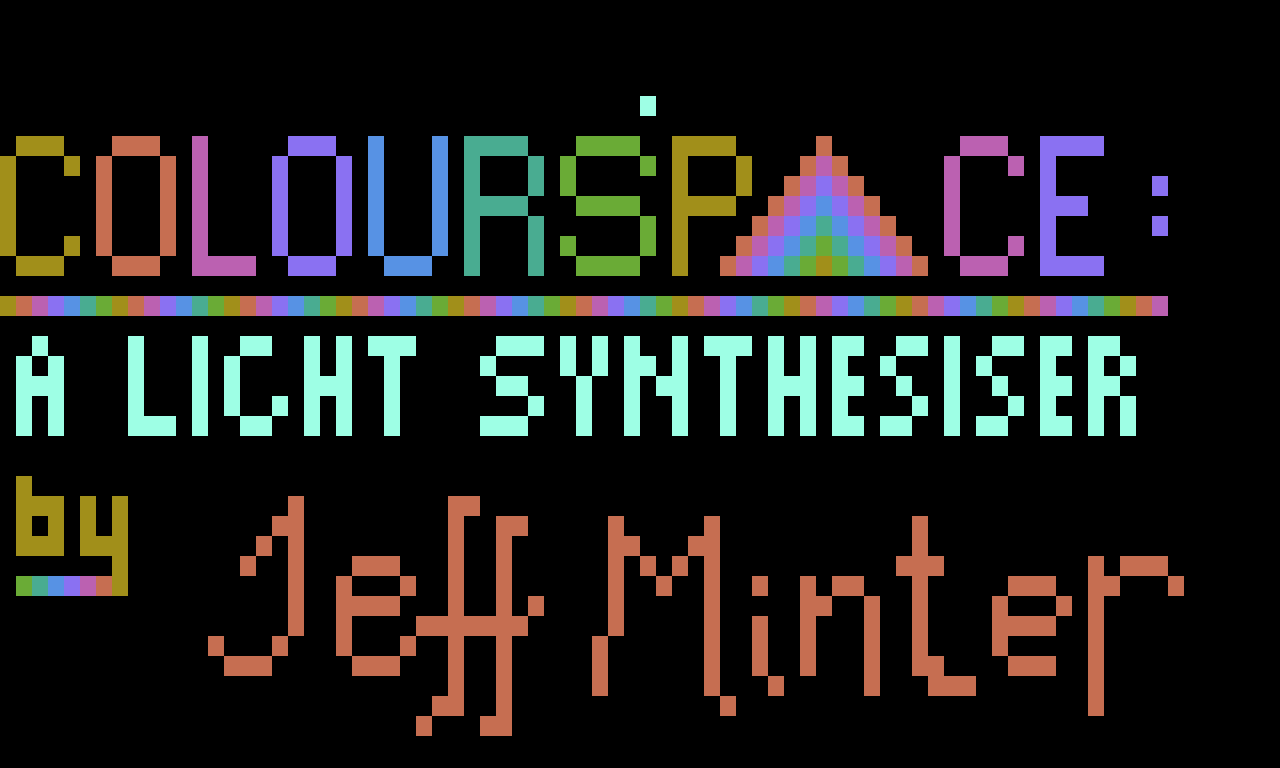
\includegraphics[width=12cm]{src/colorspace_painting/foregrounds/pixel_pattern_0.png}}%
    \end{adjustbox}
\caption{'Variable Resolution' Display Mode}
\end{figure}


%
% HIRES + HARD REFLECT
%
\clearpage
\begin{minipage}[b]{0.31\linewidth}
  \begin{figure}[H]
    {
      \setlength{\tabcolsep}{3.0pt}
      \setlength\cmidrulewidth{\heavyrulewidth} % Make cmidrule = 
      \begin{adjustbox}{height=8.5cm}

        \begin{tabular}{lll}
          \toprule
          Bytes       & Description                                                         \\
          \midrule
          \icode{\$70}  & Draw 8 Blank Lines  \\
\icode{\$70}  & Draw 8 Blank Lines  \\
\icode{\$46} \icode{\$6550} & Read 40 bytes from: \icode{\$5065} \\
\icode{\$90}  & Draw 2 Blank Lines  \\
\icode{\$4F} \icode{\$0070} & Read 40 bytes from: \icode{\$7000} \\
\icode{\$4F} \icode{\$2870} & Read 40 bytes from: \icode{\$7028} \\
\icode{\$4F} \icode{\$5070} & Read 40 bytes from: \icode{\$7050} \\
\icode{\$4F} \icode{\$7870} & Read 40 bytes from: \icode{\$7078} \\
\icode{\$4F} \icode{\$A070} & Read 40 bytes from: \icode{\$70A0} \\
\icode{\$4F} \icode{\$C870} & Read 40 bytes from: \icode{\$70C8} \\
\icode{\$4F} \icode{\$F070} & Read 40 bytes from: \icode{\$70F0} \\
\icode{\$4F} \icode{\$1871} & Read 40 bytes from: \icode{\$7118} \\
\icode{\$4F} \icode{\$4071} & Read 40 bytes from: \icode{\$7140} \\
\icode{\$4F} \icode{\$6871} & Read 40 bytes from: \icode{\$7168} \\
\icode{\$4F} \icode{\$9071} & Read 40 bytes from: \icode{\$7190} \\
\icode{\$4F} \icode{\$B871} & Read 40 bytes from: \icode{\$71B8} \\
\icode{\$4F} \icode{\$E071} & Read 40 bytes from: \icode{\$71E0} \\
\icode{\$4F} \icode{\$0872} & Read 40 bytes from: \icode{\$7208} \\
\icode{\$4F} \icode{\$3072} & Read 40 bytes from: \icode{\$7230} \\
\icode{\$4F} \icode{\$5872} & Read 40 bytes from: \icode{\$7258} \\
\icode{\$4F} \icode{\$8072} & Read 40 bytes from: \icode{\$7280} \\
\icode{\$4F} \icode{\$A872} & Read 40 bytes from: \icode{\$72A8} \\
\icode{\$4F} \icode{\$D072} & Read 40 bytes from: \icode{\$72D0} \\
\icode{\$4F} \icode{\$F872} & Read 40 bytes from: \icode{\$72F8} \\
\icode{\$4F} \icode{\$2073} & Read 40 bytes from: \icode{\$7320} \\
\icode{\$4F} \icode{\$4873} & Read 40 bytes from: \icode{\$7348} \\
\icode{\$4F} \icode{\$7073} & Read 40 bytes from: \icode{\$7370} \\
\icode{\$4F} \icode{\$9873} & Read 40 bytes from: \icode{\$7398} \\
\icode{\$4F} \icode{\$C073} & Read 40 bytes from: \icode{\$73C0} \\
\icode{\$4F} \icode{\$E873} & Read 40 bytes from: \icode{\$73E8} \\
\icode{\$4F} \icode{\$1074} & Read 40 bytes from: \icode{\$7410} \\
\icode{\$4F} \icode{\$3874} & Read 40 bytes from: \icode{\$7438} \\
\icode{\$4F} \icode{\$6074} & Read 40 bytes from: \icode{\$7460} \\
\icode{\$4F} \icode{\$8874} & Read 40 bytes from: \icode{\$7488} \\
\icode{\$4F} \icode{\$B074} & Read 40 bytes from: \icode{\$74B0} \\
\icode{\$4F} \icode{\$D874} & Read 40 bytes from: \icode{\$74D8} \\
\icode{\$4F} \icode{\$0075} & Read 40 bytes from: \icode{\$7500} \\
\icode{\$4F} \icode{\$2875} & Read 40 bytes from: \icode{\$7528} \\
\icode{\$4F} \icode{\$5075} & Read 40 bytes from: \icode{\$7550} \\
\icode{\$4F} \icode{\$7875} & Read 40 bytes from: \icode{\$7578} \\
\icode{\$4F} \icode{\$A075} & Read 40 bytes from: \icode{\$75A0} \\
\icode{\$4F} \icode{\$C875} & Read 40 bytes from: \icode{\$75C8} \\
\icode{\$4F} \icode{\$F075} & Read 40 bytes from: \icode{\$75F0} \\
\icode{\$4F} \icode{\$1876} & Read 40 bytes from: \icode{\$7618} \\
\icode{\$4F} \icode{\$4076} & Read 40 bytes from: \icode{\$7640} \\
\icode{\$4F} \icode{\$6876} & Read 40 bytes from: \icode{\$7668} \\
\icode{\$4F} \icode{\$9076} & Read 40 bytes from: \icode{\$7690} \\
\icode{\$4F} \icode{\$B876} & Read 40 bytes from: \icode{\$76B8} \\
\icode{\$4F} \icode{\$E076} & Read 40 bytes from: \icode{\$76E0} \\
\icode{\$4F} \icode{\$0877} & Read 40 bytes from: \icode{\$7708} \\
\icode{\$4F} \icode{\$3077} & Read 40 bytes from: \icode{\$7730} \\
\icode{\$4F} \icode{\$5877} & Read 40 bytes from: \icode{\$7758} \\
\icode{\$4F} \icode{\$8077} & Read 40 bytes from: \icode{\$7780} \\
\icode{\$4F} \icode{\$A877} & Read 40 bytes from: \icode{\$77A8} \\
\icode{\$4F} \icode{\$D077} & Read 40 bytes from: \icode{\$77D0} \\
\icode{\$4F} \icode{\$F877} & Read 40 bytes from: \icode{\$77F8} \\
\icode{\$4F} \icode{\$2078} & Read 40 bytes from: \icode{\$7820} \\
\icode{\$4F} \icode{\$4878} & Read 40 bytes from: \icode{\$7848} \\
\icode{\$4F} \icode{\$7078} & Read 40 bytes from: \icode{\$7870} \\
\icode{\$4F} \icode{\$9878} & Read 40 bytes from: \icode{\$7898} \\
\icode{\$4F} \icode{\$C078} & Read 40 bytes from: \icode{\$78C0} \\
\bottomrule

        \end{tabular}

      \end{adjustbox}

    }\caption*{Display List Entries: 1-61}
  \end{figure}
\end{minipage}
\hspace{0.1cm}
\begin{minipage}[b]{0.31\linewidth}
  \begin{figure}[H]
    {
      \setlength{\tabcolsep}{3.0pt}
      \setlength\cmidrulewidth{\heavyrulewidth} % Make cmidrule = 
      \begin{adjustbox}{height=8.5cm}

        \begin{tabular}{lll}
          \toprule
          Bytes       & Description                                                         \\
          \midrule
          \icode{\$4F} \icode{\$E878} & Read 40 bytes from: \icode{\$78E8} \\
\icode{\$4F} \icode{\$1079} & Read 40 bytes from: \icode{\$7910} \\
\icode{\$4F} \icode{\$3879} & Read 40 bytes from: \icode{\$7938} \\
\icode{\$4F} \icode{\$6079} & Read 40 bytes from: \icode{\$7960} \\
\icode{\$4F} \icode{\$8879} & Read 40 bytes from: \icode{\$7988} \\
\icode{\$4F} \icode{\$B079} & Read 40 bytes from: \icode{\$79B0} \\
\icode{\$4F} \icode{\$D879} & Read 40 bytes from: \icode{\$79D8} \\
\icode{\$4F} \icode{\$007A} & Read 40 bytes from: \icode{\$7A00} \\
\icode{\$4F} \icode{\$287A} & Read 40 bytes from: \icode{\$7A28} \\
\icode{\$4F} \icode{\$507A} & Read 40 bytes from: \icode{\$7A50} \\
\icode{\$4F} \icode{\$787A} & Read 40 bytes from: \icode{\$7A78} \\
\icode{\$4F} \icode{\$A07A} & Read 40 bytes from: \icode{\$7AA0} \\
\icode{\$4F} \icode{\$C87A} & Read 40 bytes from: \icode{\$7AC8} \\
\icode{\$4F} \icode{\$F07A} & Read 40 bytes from: \icode{\$7AF0} \\
\icode{\$4F} \icode{\$187B} & Read 40 bytes from: \icode{\$7B18} \\
\icode{\$4F} \icode{\$407B} & Read 40 bytes from: \icode{\$7B40} \\
\icode{\$4F} \icode{\$687B} & Read 40 bytes from: \icode{\$7B68} \\
\icode{\$4F} \icode{\$907B} & Read 40 bytes from: \icode{\$7B90} \\
\icode{\$4F} \icode{\$B87B} & Read 40 bytes from: \icode{\$7BB8} \\
\icode{\$4F} \icode{\$E07B} & Read 40 bytes from: \icode{\$7BE0} \\
\icode{\$4F} \icode{\$087C} & Read 40 bytes from: \icode{\$7C08} \\
\icode{\$4F} \icode{\$307C} & Read 40 bytes from: \icode{\$7C30} \\
\icode{\$4F} \icode{\$587C} & Read 40 bytes from: \icode{\$7C58} \\
\icode{\$4F} \icode{\$807C} & Read 40 bytes from: \icode{\$7C80} \\
\icode{\$4F} \icode{\$A87C} & Read 40 bytes from: \icode{\$7CA8} \\
\icode{\$4F} \icode{\$D07C} & Read 40 bytes from: \icode{\$7CD0} \\
\icode{\$4F} \icode{\$F87C} & Read 40 bytes from: \icode{\$7CF8} \\
\icode{\$4F} \icode{\$207D} & Read 40 bytes from: \icode{\$7D20} \\
\icode{\$4F} \icode{\$487D} & Read 40 bytes from: \icode{\$7D48} \\
\icode{\$4F} \icode{\$707D} & Read 40 bytes from: \icode{\$7D70} \\
\icode{\$4F} \icode{\$987D} & Read 40 bytes from: \icode{\$7D98} \\
\icode{\$4F} \icode{\$C07D} & Read 40 bytes from: \icode{\$7DC0} \\
\icode{\$4F} \icode{\$E87D} & Read 40 bytes from: \icode{\$7DE8} \\
\icode{\$4F} \icode{\$C07D} & Read 40 bytes from: \icode{\$7DC0} \\
\icode{\$4F} \icode{\$987D} & Read 40 bytes from: \icode{\$7D98} \\
\icode{\$4F} \icode{\$707D} & Read 40 bytes from: \icode{\$7D70} \\
\icode{\$4F} \icode{\$487D} & Read 40 bytes from: \icode{\$7D48} \\
\icode{\$4F} \icode{\$207D} & Read 40 bytes from: \icode{\$7D20} \\
\icode{\$4F} \icode{\$F87C} & Read 40 bytes from: \icode{\$7CF8} \\
\icode{\$4F} \icode{\$D07C} & Read 40 bytes from: \icode{\$7CD0} \\
\icode{\$4F} \icode{\$A87C} & Read 40 bytes from: \icode{\$7CA8} \\
\icode{\$4F} \icode{\$807C} & Read 40 bytes from: \icode{\$7C80} \\
\icode{\$4F} \icode{\$587C} & Read 40 bytes from: \icode{\$7C58} \\
\icode{\$4F} \icode{\$307C} & Read 40 bytes from: \icode{\$7C30} \\
\icode{\$4F} \icode{\$087C} & Read 40 bytes from: \icode{\$7C08} \\
\icode{\$4F} \icode{\$E07B} & Read 40 bytes from: \icode{\$7BE0} \\
\icode{\$4F} \icode{\$B87B} & Read 40 bytes from: \icode{\$7BB8} \\
\icode{\$4F} \icode{\$907B} & Read 40 bytes from: \icode{\$7B90} \\
\icode{\$4F} \icode{\$687B} & Read 40 bytes from: \icode{\$7B68} \\
\icode{\$4F} \icode{\$407B} & Read 40 bytes from: \icode{\$7B40} \\
\icode{\$4F} \icode{\$187B} & Read 40 bytes from: \icode{\$7B18} \\
\icode{\$4F} \icode{\$F07A} & Read 40 bytes from: \icode{\$7AF0} \\
\icode{\$4F} \icode{\$C87A} & Read 40 bytes from: \icode{\$7AC8} \\
\icode{\$4F} \icode{\$A07A} & Read 40 bytes from: \icode{\$7AA0} \\
\icode{\$4F} \icode{\$787A} & Read 40 bytes from: \icode{\$7A78} \\
\icode{\$4F} \icode{\$507A} & Read 40 bytes from: \icode{\$7A50} \\
\icode{\$4F} \icode{\$287A} & Read 40 bytes from: \icode{\$7A28} \\
\icode{\$4F} \icode{\$007A} & Read 40 bytes from: \icode{\$7A00} \\
\icode{\$4F} \icode{\$D879} & Read 40 bytes from: \icode{\$79D8} \\
\icode{\$4F} \icode{\$B079} & Read 40 bytes from: \icode{\$79B0} \\
\icode{\$4F} \icode{\$8879} & Read 40 bytes from: \icode{\$7988} \\
\bottomrule
%
        \end{tabular}

      \end{adjustbox}

    }\caption*{Display List Entries: 62-122}
  \end{figure}
\end{minipage}
\hspace{0.1cm}
\begin{minipage}[b]{0.31\linewidth}
  \begin{figure}[H]
    {
      \setlength{\tabcolsep}{3.0pt}
      \setlength\cmidrulewidth{\heavyrulewidth} % Make cmidrule = 
      \begin{adjustbox}{height=8.5cm}

        \begin{tabular}{lll}
          \toprule
          Bytes       & Description                                                         \\
          \midrule
          \icode{\$4F} \icode{\$6079} & Read 40 bytes from: \icode{\$7960} \\
\icode{\$4F} \icode{\$3879} & Read 40 bytes from: \icode{\$7938} \\
\icode{\$4F} \icode{\$1079} & Read 40 bytes from: \icode{\$7910} \\
\icode{\$4F} \icode{\$E878} & Read 40 bytes from: \icode{\$78E8} \\
\icode{\$4F} \icode{\$C078} & Read 40 bytes from: \icode{\$78C0} \\
\icode{\$4F} \icode{\$9878} & Read 40 bytes from: \icode{\$7898} \\
\icode{\$4F} \icode{\$7078} & Read 40 bytes from: \icode{\$7870} \\
\icode{\$4F} \icode{\$4878} & Read 40 bytes from: \icode{\$7848} \\
\icode{\$4F} \icode{\$2078} & Read 40 bytes from: \icode{\$7820} \\
\icode{\$4F} \icode{\$F877} & Read 40 bytes from: \icode{\$77F8} \\
\icode{\$4F} \icode{\$D077} & Read 40 bytes from: \icode{\$77D0} \\
\icode{\$4F} \icode{\$A877} & Read 40 bytes from: \icode{\$77A8} \\
\icode{\$4F} \icode{\$8077} & Read 40 bytes from: \icode{\$7780} \\
\icode{\$4F} \icode{\$5877} & Read 40 bytes from: \icode{\$7758} \\
\icode{\$4F} \icode{\$3077} & Read 40 bytes from: \icode{\$7730} \\
\icode{\$4F} \icode{\$0877} & Read 40 bytes from: \icode{\$7708} \\
\icode{\$4F} \icode{\$E076} & Read 40 bytes from: \icode{\$76E0} \\
\icode{\$4F} \icode{\$B876} & Read 40 bytes from: \icode{\$76B8} \\
\icode{\$4F} \icode{\$9076} & Read 40 bytes from: \icode{\$7690} \\
\icode{\$4F} \icode{\$6876} & Read 40 bytes from: \icode{\$7668} \\
\icode{\$4F} \icode{\$4076} & Read 40 bytes from: \icode{\$7640} \\
\icode{\$4F} \icode{\$1876} & Read 40 bytes from: \icode{\$7618} \\
\icode{\$4F} \icode{\$F075} & Read 40 bytes from: \icode{\$75F0} \\
\icode{\$4F} \icode{\$C875} & Read 40 bytes from: \icode{\$75C8} \\
\icode{\$4F} \icode{\$A075} & Read 40 bytes from: \icode{\$75A0} \\
\icode{\$4F} \icode{\$7875} & Read 40 bytes from: \icode{\$7578} \\
\icode{\$4F} \icode{\$5075} & Read 40 bytes from: \icode{\$7550} \\
\icode{\$4F} \icode{\$2875} & Read 40 bytes from: \icode{\$7528} \\
\icode{\$4F} \icode{\$0075} & Read 40 bytes from: \icode{\$7500} \\
\icode{\$4F} \icode{\$D874} & Read 40 bytes from: \icode{\$74D8} \\
\icode{\$4F} \icode{\$B074} & Read 40 bytes from: \icode{\$74B0} \\
\icode{\$4F} \icode{\$8874} & Read 40 bytes from: \icode{\$7488} \\
\icode{\$4F} \icode{\$6074} & Read 40 bytes from: \icode{\$7460} \\
\icode{\$4F} \icode{\$3874} & Read 40 bytes from: \icode{\$7438} \\
\icode{\$4F} \icode{\$1074} & Read 40 bytes from: \icode{\$7410} \\
\icode{\$4F} \icode{\$E873} & Read 40 bytes from: \icode{\$73E8} \\
\icode{\$4F} \icode{\$C073} & Read 40 bytes from: \icode{\$73C0} \\
\icode{\$4F} \icode{\$9873} & Read 40 bytes from: \icode{\$7398} \\
\icode{\$4F} \icode{\$7073} & Read 40 bytes from: \icode{\$7370} \\
\icode{\$4F} \icode{\$4873} & Read 40 bytes from: \icode{\$7348} \\
\icode{\$4F} \icode{\$2073} & Read 40 bytes from: \icode{\$7320} \\
\icode{\$4F} \icode{\$F872} & Read 40 bytes from: \icode{\$72F8} \\
\icode{\$4F} \icode{\$D072} & Read 40 bytes from: \icode{\$72D0} \\
\icode{\$4F} \icode{\$A872} & Read 40 bytes from: \icode{\$72A8} \\
\icode{\$4F} \icode{\$8072} & Read 40 bytes from: \icode{\$7280} \\
\icode{\$4F} \icode{\$5872} & Read 40 bytes from: \icode{\$7258} \\
\icode{\$4F} \icode{\$3072} & Read 40 bytes from: \icode{\$7230} \\
\icode{\$4F} \icode{\$0872} & Read 40 bytes from: \icode{\$7208} \\
\icode{\$4F} \icode{\$E071} & Read 40 bytes from: \icode{\$71E0} \\
\icode{\$4F} \icode{\$B871} & Read 40 bytes from: \icode{\$71B8} \\
\icode{\$4F} \icode{\$9071} & Read 40 bytes from: \icode{\$7190} \\
\icode{\$4F} \icode{\$6871} & Read 40 bytes from: \icode{\$7168} \\
\icode{\$4F} \icode{\$4071} & Read 40 bytes from: \icode{\$7140} \\
\icode{\$4F} \icode{\$1871} & Read 40 bytes from: \icode{\$7118} \\
\icode{\$4F} \icode{\$F070} & Read 40 bytes from: \icode{\$70F0} \\
\icode{\$4F} \icode{\$C870} & Read 40 bytes from: \icode{\$70C8} \\
\icode{\$4F} \icode{\$A070} & Read 40 bytes from: \icode{\$70A0} \\
\icode{\$4F} \icode{\$7870} & Read 40 bytes from: \icode{\$7078} \\
\icode{\$4F} \icode{\$5070} & Read 40 bytes from: \icode{\$7050} \\
\icode{\$4F} \icode{\$2870} & Read 40 bytes from: \icode{\$7028} \\
\bottomrule
%
        \end{tabular}

      \end{adjustbox}

    }\caption*{Display List Entries: 123-182}
  \end{figure}
\end{minipage}

\clearpage
\begin{figure}[H]
    \centering
    \begin{adjustbox}{width=12cm,center}
      \frame{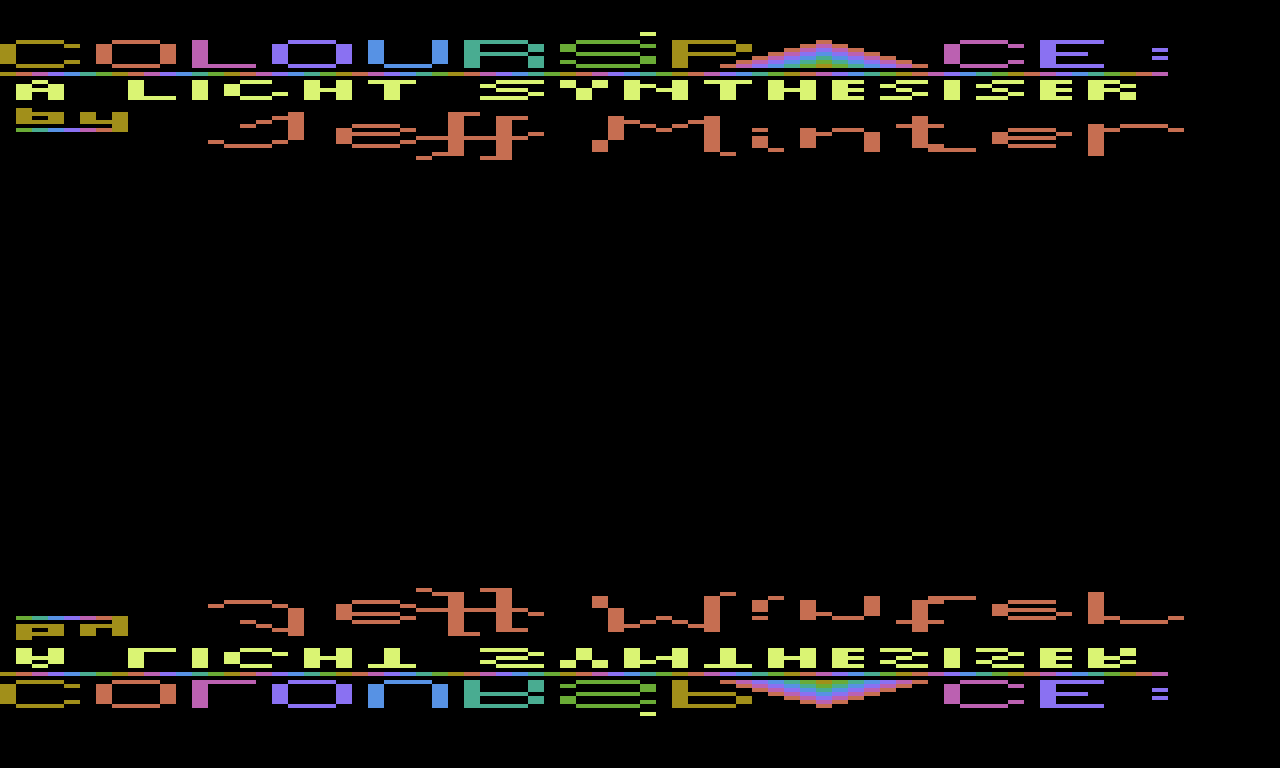
\includegraphics[width=12cm]{src/colorspace_painting/foregrounds/pixel_pattern_1.png}}%
    \end{adjustbox}
\caption{'Hi-Resolution + Hard Reflect' Display Mode}
\end{figure}


%
% CURVED COLORSPACE 1
%
\clearpage
\begin{minipage}[b]{0.31\linewidth}
  \begin{figure}[H]
    {
      \setlength{\tabcolsep}{3.0pt}
      \setlength\cmidrulewidth{\heavyrulewidth} % Make cmidrule = 
      \begin{adjustbox}{height=8.5cm}

        \begin{tabular}{lll}
          \toprule
          Bytes       & Description                                                         \\
          \midrule
          \icode{\$70}  & Draw 8 Blank Lines  \\
\icode{\$70}  & Draw 8 Blank Lines  \\
\icode{\$46} \icode{\$7950} & Read 40 bytes from: \icode{\$5079} \\
\icode{\$90}  & Draw 2 Blank Lines  \\
\icode{\$4F} \icode{\$0070} & Read 40 bytes from: \icode{\$7000} \\
\icode{\$4F} \icode{\$2870} & Read 40 bytes from: \icode{\$7028} \\
\icode{\$4F} \icode{\$5070} & Read 40 bytes from: \icode{\$7050} \\
\icode{\$4F} \icode{\$7870} & Read 40 bytes from: \icode{\$7078} \\
\icode{\$4F} \icode{\$A070} & Read 40 bytes from: \icode{\$70A0} \\
\icode{\$4F} \icode{\$A070} & Read 40 bytes from: \icode{\$70A0} \\
\icode{\$4F} \icode{\$C870} & Read 40 bytes from: \icode{\$70C8} \\
\icode{\$4F} \icode{\$C870} & Read 40 bytes from: \icode{\$70C8} \\
\icode{\$4F} \icode{\$F070} & Read 40 bytes from: \icode{\$70F0} \\
\icode{\$4F} \icode{\$F070} & Read 40 bytes from: \icode{\$70F0} \\
\icode{\$4F} \icode{\$1871} & Read 40 bytes from: \icode{\$7118} \\
\icode{\$4F} \icode{\$1871} & Read 40 bytes from: \icode{\$7118} \\
\icode{\$4F} \icode{\$4071} & Read 40 bytes from: \icode{\$7140} \\
\icode{\$4F} \icode{\$4071} & Read 40 bytes from: \icode{\$7140} \\
\icode{\$4F} \icode{\$4071} & Read 40 bytes from: \icode{\$7140} \\
\icode{\$4F} \icode{\$6871} & Read 40 bytes from: \icode{\$7168} \\
\icode{\$4F} \icode{\$6871} & Read 40 bytes from: \icode{\$7168} \\
\icode{\$4F} \icode{\$6871} & Read 40 bytes from: \icode{\$7168} \\
\icode{\$4F} \icode{\$9071} & Read 40 bytes from: \icode{\$7190} \\
\icode{\$4F} \icode{\$9071} & Read 40 bytes from: \icode{\$7190} \\
\icode{\$4F} \icode{\$9071} & Read 40 bytes from: \icode{\$7190} \\
\icode{\$4F} \icode{\$B871} & Read 40 bytes from: \icode{\$71B8} \\
\icode{\$4F} \icode{\$B871} & Read 40 bytes from: \icode{\$71B8} \\
\icode{\$4F} \icode{\$B871} & Read 40 bytes from: \icode{\$71B8} \\
\icode{\$4F} \icode{\$E071} & Read 40 bytes from: \icode{\$71E0} \\
\icode{\$4F} \icode{\$E071} & Read 40 bytes from: \icode{\$71E0} \\
\icode{\$4F} \icode{\$E071} & Read 40 bytes from: \icode{\$71E0} \\
\icode{\$4F} \icode{\$E071} & Read 40 bytes from: \icode{\$71E0} \\
\icode{\$4F} \icode{\$0872} & Read 40 bytes from: \icode{\$7208} \\
\icode{\$4F} \icode{\$0872} & Read 40 bytes from: \icode{\$7208} \\
\icode{\$4F} \icode{\$0872} & Read 40 bytes from: \icode{\$7208} \\
\icode{\$4F} \icode{\$0872} & Read 40 bytes from: \icode{\$7208} \\
\icode{\$4F} \icode{\$3072} & Read 40 bytes from: \icode{\$7230} \\
\icode{\$4F} \icode{\$3072} & Read 40 bytes from: \icode{\$7230} \\
\icode{\$4F} \icode{\$3072} & Read 40 bytes from: \icode{\$7230} \\
\icode{\$4F} \icode{\$3072} & Read 40 bytes from: \icode{\$7230} \\
\icode{\$4F} \icode{\$5872} & Read 40 bytes from: \icode{\$7258} \\
\icode{\$4F} \icode{\$5872} & Read 40 bytes from: \icode{\$7258} \\
\icode{\$4F} \icode{\$5872} & Read 40 bytes from: \icode{\$7258} \\
\icode{\$4F} \icode{\$5872} & Read 40 bytes from: \icode{\$7258} \\
\icode{\$4F} \icode{\$8072} & Read 40 bytes from: \icode{\$7280} \\
\icode{\$4F} \icode{\$8072} & Read 40 bytes from: \icode{\$7280} \\
\icode{\$4F} \icode{\$8072} & Read 40 bytes from: \icode{\$7280} \\
\icode{\$4F} \icode{\$8072} & Read 40 bytes from: \icode{\$7280} \\
\icode{\$4F} \icode{\$8072} & Read 40 bytes from: \icode{\$7280} \\
\icode{\$4F} \icode{\$A872} & Read 40 bytes from: \icode{\$72A8} \\
\icode{\$4F} \icode{\$A872} & Read 40 bytes from: \icode{\$72A8} \\
\icode{\$4F} \icode{\$A872} & Read 40 bytes from: \icode{\$72A8} \\
\icode{\$4F} \icode{\$A872} & Read 40 bytes from: \icode{\$72A8} \\
\icode{\$4F} \icode{\$A872} & Read 40 bytes from: \icode{\$72A8} \\
\icode{\$4F} \icode{\$D072} & Read 40 bytes from: \icode{\$72D0} \\
\icode{\$4F} \icode{\$D072} & Read 40 bytes from: \icode{\$72D0} \\
\icode{\$4F} \icode{\$D072} & Read 40 bytes from: \icode{\$72D0} \\
\icode{\$4F} \icode{\$D072} & Read 40 bytes from: \icode{\$72D0} \\
\icode{\$4F} \icode{\$D072} & Read 40 bytes from: \icode{\$72D0} \\
\icode{\$4F} \icode{\$F872} & Read 40 bytes from: \icode{\$72F8} \\
\icode{\$4F} \icode{\$F872} & Read 40 bytes from: \icode{\$72F8} \\
\bottomrule

        \end{tabular}

      \end{adjustbox}

    }\caption*{Display List Entries: 1-61}
  \end{figure}
\end{minipage}
\hspace{0.1cm}
\begin{minipage}[b]{0.31\linewidth}
  \begin{figure}[H]
    {
      \setlength{\tabcolsep}{3.0pt}
      \setlength\cmidrulewidth{\heavyrulewidth} % Make cmidrule = 
      \begin{adjustbox}{height=8.5cm}

        \begin{tabular}{lll}
          \toprule
          Bytes       & Description                                                         \\
          \midrule
          \icode{\$4F} \icode{\$F872} & Read 40 bytes from: \icode{\$72F8} \\
\icode{\$4F} \icode{\$F872} & Read 40 bytes from: \icode{\$72F8} \\
\icode{\$4F} \icode{\$F872} & Read 40 bytes from: \icode{\$72F8} \\
\icode{\$4F} \icode{\$2073} & Read 40 bytes from: \icode{\$7320} \\
\icode{\$4F} \icode{\$2073} & Read 40 bytes from: \icode{\$7320} \\
\icode{\$4F} \icode{\$2073} & Read 40 bytes from: \icode{\$7320} \\
\icode{\$4F} \icode{\$2073} & Read 40 bytes from: \icode{\$7320} \\
\icode{\$4F} \icode{\$2073} & Read 40 bytes from: \icode{\$7320} \\
\icode{\$4F} \icode{\$2073} & Read 40 bytes from: \icode{\$7320} \\
\icode{\$4F} \icode{\$4873} & Read 40 bytes from: \icode{\$7348} \\
\icode{\$4F} \icode{\$4873} & Read 40 bytes from: \icode{\$7348} \\
\icode{\$4F} \icode{\$4873} & Read 40 bytes from: \icode{\$7348} \\
\icode{\$4F} \icode{\$4873} & Read 40 bytes from: \icode{\$7348} \\
\icode{\$4F} \icode{\$4873} & Read 40 bytes from: \icode{\$7348} \\
\icode{\$4F} \icode{\$4873} & Read 40 bytes from: \icode{\$7348} \\
\icode{\$4F} \icode{\$7073} & Read 40 bytes from: \icode{\$7370} \\
\icode{\$4F} \icode{\$7073} & Read 40 bytes from: \icode{\$7370} \\
\icode{\$4F} \icode{\$7073} & Read 40 bytes from: \icode{\$7370} \\
\icode{\$4F} \icode{\$7073} & Read 40 bytes from: \icode{\$7370} \\
\icode{\$4F} \icode{\$7073} & Read 40 bytes from: \icode{\$7370} \\
\icode{\$4F} \icode{\$7073} & Read 40 bytes from: \icode{\$7370} \\
\icode{\$4F} \icode{\$9873} & Read 40 bytes from: \icode{\$7398} \\
\icode{\$4F} \icode{\$9873} & Read 40 bytes from: \icode{\$7398} \\
\icode{\$4F} \icode{\$9873} & Read 40 bytes from: \icode{\$7398} \\
\icode{\$4F} \icode{\$9873} & Read 40 bytes from: \icode{\$7398} \\
\icode{\$4F} \icode{\$9873} & Read 40 bytes from: \icode{\$7398} \\
\icode{\$4F} \icode{\$9873} & Read 40 bytes from: \icode{\$7398} \\
\icode{\$4F} \icode{\$C073} & Read 40 bytes from: \icode{\$73C0} \\
\icode{\$4F} \icode{\$C073} & Read 40 bytes from: \icode{\$73C0} \\
\icode{\$4F} \icode{\$C073} & Read 40 bytes from: \icode{\$73C0} \\
\icode{\$4F} \icode{\$C073} & Read 40 bytes from: \icode{\$73C0} \\
\icode{\$4F} \icode{\$C073} & Read 40 bytes from: \icode{\$73C0} \\
\icode{\$4F} \icode{\$C073} & Read 40 bytes from: \icode{\$73C0} \\
\icode{\$4F} \icode{\$C073} & Read 40 bytes from: \icode{\$73C0} \\
\icode{\$4F} \icode{\$E873} & Read 40 bytes from: \icode{\$73E8} \\
\icode{\$4F} \icode{\$E873} & Read 40 bytes from: \icode{\$73E8} \\
\icode{\$4F} \icode{\$E873} & Read 40 bytes from: \icode{\$73E8} \\
\icode{\$4F} \icode{\$E873} & Read 40 bytes from: \icode{\$73E8} \\
\icode{\$4F} \icode{\$E873} & Read 40 bytes from: \icode{\$73E8} \\
\icode{\$4F} \icode{\$E873} & Read 40 bytes from: \icode{\$73E8} \\
\icode{\$4F} \icode{\$E873} & Read 40 bytes from: \icode{\$73E8} \\
\icode{\$4F} \icode{\$1074} & Read 40 bytes from: \icode{\$7410} \\
\icode{\$4F} \icode{\$1074} & Read 40 bytes from: \icode{\$7410} \\
\icode{\$4F} \icode{\$1074} & Read 40 bytes from: \icode{\$7410} \\
\icode{\$4F} \icode{\$1074} & Read 40 bytes from: \icode{\$7410} \\
\icode{\$4F} \icode{\$1074} & Read 40 bytes from: \icode{\$7410} \\
\icode{\$4F} \icode{\$1074} & Read 40 bytes from: \icode{\$7410} \\
\icode{\$4F} \icode{\$1074} & Read 40 bytes from: \icode{\$7410} \\
\icode{\$4F} \icode{\$3874} & Read 40 bytes from: \icode{\$7438} \\
\icode{\$4F} \icode{\$3874} & Read 40 bytes from: \icode{\$7438} \\
\icode{\$4F} \icode{\$3874} & Read 40 bytes from: \icode{\$7438} \\
\icode{\$4F} \icode{\$3874} & Read 40 bytes from: \icode{\$7438} \\
\icode{\$4F} \icode{\$3874} & Read 40 bytes from: \icode{\$7438} \\
\icode{\$4F} \icode{\$3874} & Read 40 bytes from: \icode{\$7438} \\
\icode{\$4F} \icode{\$3874} & Read 40 bytes from: \icode{\$7438} \\
\icode{\$4F} \icode{\$6074} & Read 40 bytes from: \icode{\$7460} \\
\icode{\$4F} \icode{\$6074} & Read 40 bytes from: \icode{\$7460} \\
\icode{\$4F} \icode{\$6074} & Read 40 bytes from: \icode{\$7460} \\
\icode{\$4F} \icode{\$6074} & Read 40 bytes from: \icode{\$7460} \\
\icode{\$4F} \icode{\$6074} & Read 40 bytes from: \icode{\$7460} \\
\icode{\$4F} \icode{\$6074} & Read 40 bytes from: \icode{\$7460} \\
\bottomrule
%
        \end{tabular}

      \end{adjustbox}

    }\caption*{Display List Entries: 62-122}
  \end{figure}
\end{minipage}
\hspace{0.1cm}
\begin{minipage}[b]{0.31\linewidth}
  \begin{figure}[H]
    {
      \setlength{\tabcolsep}{3.0pt}
      \setlength\cmidrulewidth{\heavyrulewidth} % Make cmidrule = 
      \begin{adjustbox}{height=8.5cm}

        \begin{tabular}{lll}
          \toprule
          Bytes       & Description                                                         \\
          \midrule
          \icode{\$4F} \icode{\$6074} & Read 40 bytes from: \icode{\$7460} \\
\icode{\$4F} \icode{\$6074} & Read 40 bytes from: \icode{\$7460} \\
\icode{\$4F} \icode{\$8874} & Read 40 bytes from: \icode{\$7488} \\
\icode{\$4F} \icode{\$8874} & Read 40 bytes from: \icode{\$7488} \\
\icode{\$4F} \icode{\$8874} & Read 40 bytes from: \icode{\$7488} \\
\icode{\$4F} \icode{\$8874} & Read 40 bytes from: \icode{\$7488} \\
\icode{\$4F} \icode{\$8874} & Read 40 bytes from: \icode{\$7488} \\
\icode{\$4F} \icode{\$8874} & Read 40 bytes from: \icode{\$7488} \\
\icode{\$4F} \icode{\$8874} & Read 40 bytes from: \icode{\$7488} \\
\icode{\$4F} \icode{\$8874} & Read 40 bytes from: \icode{\$7488} \\
\icode{\$4F} \icode{\$B074} & Read 40 bytes from: \icode{\$74B0} \\
\icode{\$4F} \icode{\$B074} & Read 40 bytes from: \icode{\$74B0} \\
\icode{\$4F} \icode{\$B074} & Read 40 bytes from: \icode{\$74B0} \\
\icode{\$4F} \icode{\$B074} & Read 40 bytes from: \icode{\$74B0} \\
\icode{\$4F} \icode{\$B074} & Read 40 bytes from: \icode{\$74B0} \\
\icode{\$4F} \icode{\$B074} & Read 40 bytes from: \icode{\$74B0} \\
\icode{\$4F} \icode{\$B074} & Read 40 bytes from: \icode{\$74B0} \\
\icode{\$4F} \icode{\$B074} & Read 40 bytes from: \icode{\$74B0} \\
\icode{\$4F} \icode{\$D874} & Read 40 bytes from: \icode{\$74D8} \\
\icode{\$4F} \icode{\$D874} & Read 40 bytes from: \icode{\$74D8} \\
\icode{\$4F} \icode{\$D874} & Read 40 bytes from: \icode{\$74D8} \\
\icode{\$4F} \icode{\$D874} & Read 40 bytes from: \icode{\$74D8} \\
\icode{\$4F} \icode{\$D874} & Read 40 bytes from: \icode{\$74D8} \\
\icode{\$4F} \icode{\$D874} & Read 40 bytes from: \icode{\$74D8} \\
\icode{\$4F} \icode{\$D874} & Read 40 bytes from: \icode{\$74D8} \\
\icode{\$4F} \icode{\$D874} & Read 40 bytes from: \icode{\$74D8} \\
\icode{\$4F} \icode{\$0075} & Read 40 bytes from: \icode{\$7500} \\
\icode{\$4F} \icode{\$0075} & Read 40 bytes from: \icode{\$7500} \\
\icode{\$4F} \icode{\$0075} & Read 40 bytes from: \icode{\$7500} \\
\icode{\$4F} \icode{\$0075} & Read 40 bytes from: \icode{\$7500} \\
\icode{\$4F} \icode{\$0075} & Read 40 bytes from: \icode{\$7500} \\
\icode{\$4F} \icode{\$0075} & Read 40 bytes from: \icode{\$7500} \\
\icode{\$4F} \icode{\$0075} & Read 40 bytes from: \icode{\$7500} \\
\icode{\$4F} \icode{\$0075} & Read 40 bytes from: \icode{\$7500} \\
\icode{\$4F} \icode{\$0075} & Read 40 bytes from: \icode{\$7500} \\
\icode{\$4F} \icode{\$2875} & Read 40 bytes from: \icode{\$7528} \\
\icode{\$4F} \icode{\$2875} & Read 40 bytes from: \icode{\$7528} \\
\icode{\$4F} \icode{\$2875} & Read 40 bytes from: \icode{\$7528} \\
\icode{\$4F} \icode{\$2875} & Read 40 bytes from: \icode{\$7528} \\
\icode{\$4F} \icode{\$2875} & Read 40 bytes from: \icode{\$7528} \\
\icode{\$4F} \icode{\$2875} & Read 40 bytes from: \icode{\$7528} \\
\icode{\$4F} \icode{\$2875} & Read 40 bytes from: \icode{\$7528} \\
\icode{\$4F} \icode{\$2875} & Read 40 bytes from: \icode{\$7528} \\
\icode{\$4F} \icode{\$2875} & Read 40 bytes from: \icode{\$7528} \\
\icode{\$4F} \icode{\$5075} & Read 40 bytes from: \icode{\$7550} \\
\icode{\$4F} \icode{\$5075} & Read 40 bytes from: \icode{\$7550} \\
\icode{\$4F} \icode{\$5075} & Read 40 bytes from: \icode{\$7550} \\
\icode{\$4F} \icode{\$5075} & Read 40 bytes from: \icode{\$7550} \\
\icode{\$4F} \icode{\$5075} & Read 40 bytes from: \icode{\$7550} \\
\icode{\$4F} \icode{\$5075} & Read 40 bytes from: \icode{\$7550} \\
\icode{\$4F} \icode{\$5075} & Read 40 bytes from: \icode{\$7550} \\
\icode{\$4F} \icode{\$5075} & Read 40 bytes from: \icode{\$7550} \\
\icode{\$4F} \icode{\$5075} & Read 40 bytes from: \icode{\$7550} \\
\icode{\$4F} \icode{\$7875} & Read 40 bytes from: \icode{\$7578} \\
\icode{\$4F} \icode{\$7875} & Read 40 bytes from: \icode{\$7578} \\
\icode{\$4F} \icode{\$7875} & Read 40 bytes from: \icode{\$7578} \\
\icode{\$4F} \icode{\$7875} & Read 40 bytes from: \icode{\$7578} \\
\icode{\$4F} \icode{\$7875} & Read 40 bytes from: \icode{\$7578} \\
\icode{\$4F} \icode{\$7875} & Read 40 bytes from: \icode{\$7578} \\
\icode{\$4F} \icode{\$7875} & Read 40 bytes from: \icode{\$7578} \\
\icode{\$4F} \icode{\$7875} & Read 40 bytes from: \icode{\$7578} \\
\icode{\$4F} \icode{\$7875} & Read 40 bytes from: \icode{\$7578} \\
\bottomrule
%
        \end{tabular}

      \end{adjustbox}

    }\caption*{Display List Entries: 123-182}
  \end{figure}
\end{minipage}

\clearpage
\begin{figure}[H]
    \centering
    \begin{adjustbox}{width=12cm,center}
      \frame{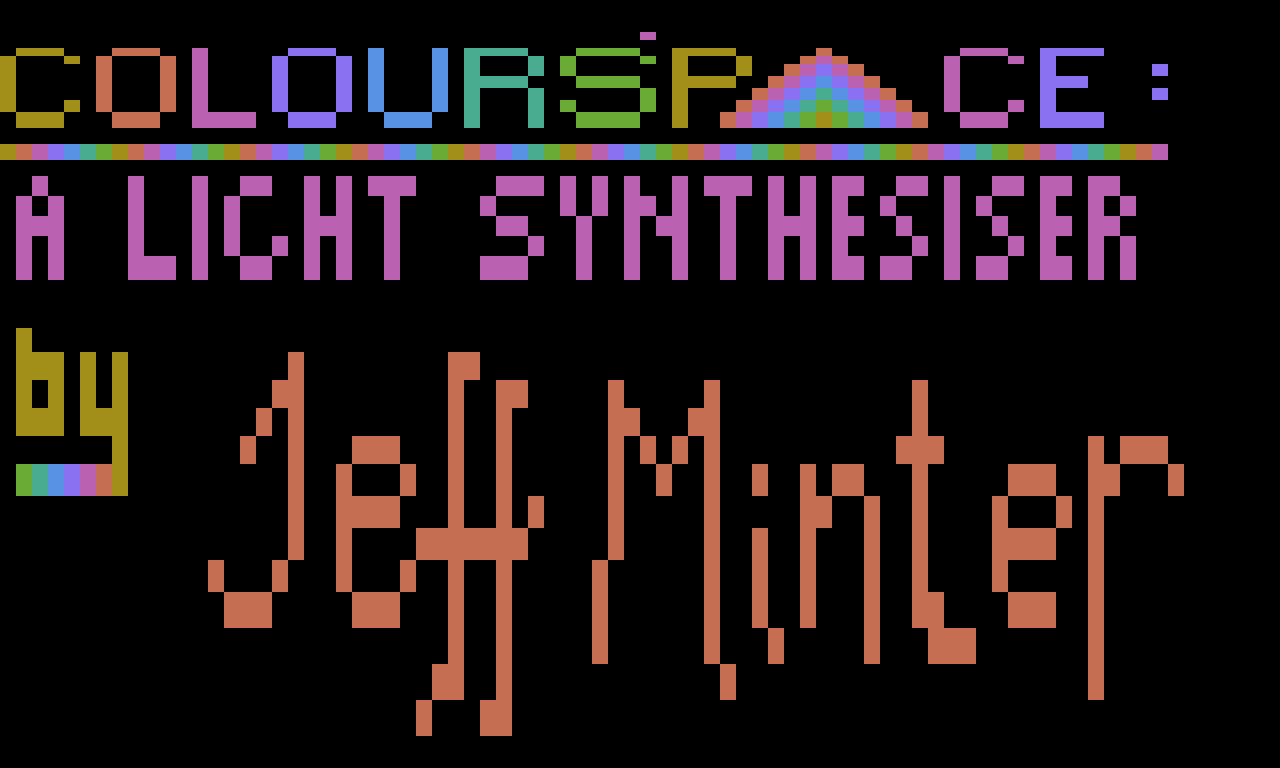
\includegraphics[width=12cm]{src/colorspace_painting/foregrounds/pixel_pattern_2.png}}%
    \end{adjustbox}
\caption{'Curved Colourspace 1' Display Mode}
\end{figure}


%
% CURVED COLORSPACE 2
%
\clearpage
\begin{minipage}[b]{0.31\linewidth}
  \begin{figure}[H]
    {
      \setlength{\tabcolsep}{3.0pt}
      \setlength\cmidrulewidth{\heavyrulewidth} % Make cmidrule = 
      \begin{adjustbox}{height=8.5cm}

        \begin{tabular}{lll}
          \toprule
          Bytes       & Description                                                         \\
          \midrule
          \icode{\$70}  & Draw 8 Blank Lines  \\
\icode{\$70}  & Draw 8 Blank Lines  \\
\icode{\$46} \icode{\$8D50} & Read 40 bytes from: \icode{\$508D} \\
\icode{\$90}  & Draw 2 Blank Lines  \\
\icode{\$4F} \icode{\$0070} & Read 40 bytes from: \icode{\$7000} \\
\icode{\$4F} \icode{\$2870} & Read 40 bytes from: \icode{\$7028} \\
\icode{\$4F} \icode{\$5070} & Read 40 bytes from: \icode{\$7050} \\
\icode{\$4F} \icode{\$5070} & Read 40 bytes from: \icode{\$7050} \\
\icode{\$4F} \icode{\$7870} & Read 40 bytes from: \icode{\$7078} \\
\icode{\$4F} \icode{\$7870} & Read 40 bytes from: \icode{\$7078} \\
\icode{\$4F} \icode{\$A070} & Read 40 bytes from: \icode{\$70A0} \\
\icode{\$4F} \icode{\$A070} & Read 40 bytes from: \icode{\$70A0} \\
\icode{\$4F} \icode{\$A070} & Read 40 bytes from: \icode{\$70A0} \\
\icode{\$4F} \icode{\$C870} & Read 40 bytes from: \icode{\$70C8} \\
\icode{\$4F} \icode{\$C870} & Read 40 bytes from: \icode{\$70C8} \\
\icode{\$4F} \icode{\$C870} & Read 40 bytes from: \icode{\$70C8} \\
\icode{\$4F} \icode{\$F070} & Read 40 bytes from: \icode{\$70F0} \\
\icode{\$4F} \icode{\$F070} & Read 40 bytes from: \icode{\$70F0} \\
\icode{\$4F} \icode{\$F070} & Read 40 bytes from: \icode{\$70F0} \\
\icode{\$4F} \icode{\$F070} & Read 40 bytes from: \icode{\$70F0} \\
\icode{\$4F} \icode{\$1871} & Read 40 bytes from: \icode{\$7118} \\
\icode{\$4F} \icode{\$1871} & Read 40 bytes from: \icode{\$7118} \\
\icode{\$4F} \icode{\$1871} & Read 40 bytes from: \icode{\$7118} \\
\icode{\$4F} \icode{\$1871} & Read 40 bytes from: \icode{\$7118} \\
\icode{\$4F} \icode{\$4071} & Read 40 bytes from: \icode{\$7140} \\
\icode{\$4F} \icode{\$4071} & Read 40 bytes from: \icode{\$7140} \\
\icode{\$4F} \icode{\$4071} & Read 40 bytes from: \icode{\$7140} \\
\icode{\$4F} \icode{\$4071} & Read 40 bytes from: \icode{\$7140} \\
\icode{\$4F} \icode{\$4071} & Read 40 bytes from: \icode{\$7140} \\
\icode{\$4F} \icode{\$6871} & Read 40 bytes from: \icode{\$7168} \\
\icode{\$4F} \icode{\$6871} & Read 40 bytes from: \icode{\$7168} \\
\icode{\$4F} \icode{\$6871} & Read 40 bytes from: \icode{\$7168} \\
\icode{\$4F} \icode{\$6871} & Read 40 bytes from: \icode{\$7168} \\
\icode{\$4F} \icode{\$6871} & Read 40 bytes from: \icode{\$7168} \\
\icode{\$4F} \icode{\$9071} & Read 40 bytes from: \icode{\$7190} \\
\icode{\$4F} \icode{\$9071} & Read 40 bytes from: \icode{\$7190} \\
\icode{\$4F} \icode{\$9071} & Read 40 bytes from: \icode{\$7190} \\
\icode{\$4F} \icode{\$9071} & Read 40 bytes from: \icode{\$7190} \\
\icode{\$4F} \icode{\$9071} & Read 40 bytes from: \icode{\$7190} \\
\icode{\$4F} \icode{\$9071} & Read 40 bytes from: \icode{\$7190} \\
\icode{\$4F} \icode{\$B871} & Read 40 bytes from: \icode{\$71B8} \\
\icode{\$4F} \icode{\$B871} & Read 40 bytes from: \icode{\$71B8} \\
\icode{\$4F} \icode{\$B871} & Read 40 bytes from: \icode{\$71B8} \\
\icode{\$4F} \icode{\$B871} & Read 40 bytes from: \icode{\$71B8} \\
\icode{\$4F} \icode{\$B871} & Read 40 bytes from: \icode{\$71B8} \\
\icode{\$4F} \icode{\$B871} & Read 40 bytes from: \icode{\$71B8} \\
\icode{\$4F} \icode{\$E071} & Read 40 bytes from: \icode{\$71E0} \\
\icode{\$4F} \icode{\$E071} & Read 40 bytes from: \icode{\$71E0} \\
\icode{\$4F} \icode{\$E071} & Read 40 bytes from: \icode{\$71E0} \\
\icode{\$4F} \icode{\$E071} & Read 40 bytes from: \icode{\$71E0} \\
\icode{\$4F} \icode{\$E071} & Read 40 bytes from: \icode{\$71E0} \\
\icode{\$4F} \icode{\$E071} & Read 40 bytes from: \icode{\$71E0} \\
\icode{\$4F} \icode{\$E071} & Read 40 bytes from: \icode{\$71E0} \\
\icode{\$4F} \icode{\$0872} & Read 40 bytes from: \icode{\$7208} \\
\icode{\$4F} \icode{\$0872} & Read 40 bytes from: \icode{\$7208} \\
\icode{\$4F} \icode{\$0872} & Read 40 bytes from: \icode{\$7208} \\
\icode{\$4F} \icode{\$0872} & Read 40 bytes from: \icode{\$7208} \\
\icode{\$4F} \icode{\$0872} & Read 40 bytes from: \icode{\$7208} \\
\icode{\$4F} \icode{\$0872} & Read 40 bytes from: \icode{\$7208} \\
\icode{\$4F} \icode{\$0872} & Read 40 bytes from: \icode{\$7208} \\
\icode{\$4F} \icode{\$3072} & Read 40 bytes from: \icode{\$7230} \\
\bottomrule

        \end{tabular}

      \end{adjustbox}

    }\caption*{Display List Entries: 1-61}
  \end{figure}
\end{minipage}
\hspace{0.1cm}
\begin{minipage}[b]{0.31\linewidth}
  \begin{figure}[H]
    {
      \setlength{\tabcolsep}{3.0pt}
      \setlength\cmidrulewidth{\heavyrulewidth} % Make cmidrule = 
      \begin{adjustbox}{height=8.5cm}

        \begin{tabular}{lll}
          \toprule
          Bytes       & Description                                                         \\
          \midrule
          \icode{\$4F} \icode{\$3072} & Read 40 bytes from: \icode{\$7230} \\
\icode{\$4F} \icode{\$3072} & Read 40 bytes from: \icode{\$7230} \\
\icode{\$4F} \icode{\$3072} & Read 40 bytes from: \icode{\$7230} \\
\icode{\$4F} \icode{\$3072} & Read 40 bytes from: \icode{\$7230} \\
\icode{\$4F} \icode{\$3072} & Read 40 bytes from: \icode{\$7230} \\
\icode{\$4F} \icode{\$3072} & Read 40 bytes from: \icode{\$7230} \\
\icode{\$4F} \icode{\$3072} & Read 40 bytes from: \icode{\$7230} \\
\icode{\$4F} \icode{\$5872} & Read 40 bytes from: \icode{\$7258} \\
\icode{\$4F} \icode{\$5872} & Read 40 bytes from: \icode{\$7258} \\
\icode{\$4F} \icode{\$5872} & Read 40 bytes from: \icode{\$7258} \\
\icode{\$4F} \icode{\$5872} & Read 40 bytes from: \icode{\$7258} \\
\icode{\$4F} \icode{\$5872} & Read 40 bytes from: \icode{\$7258} \\
\icode{\$4F} \icode{\$5872} & Read 40 bytes from: \icode{\$7258} \\
\icode{\$4F} \icode{\$5872} & Read 40 bytes from: \icode{\$7258} \\
\icode{\$4F} \icode{\$5872} & Read 40 bytes from: \icode{\$7258} \\
\icode{\$4F} \icode{\$8072} & Read 40 bytes from: \icode{\$7280} \\
\icode{\$4F} \icode{\$8072} & Read 40 bytes from: \icode{\$7280} \\
\icode{\$4F} \icode{\$8072} & Read 40 bytes from: \icode{\$7280} \\
\icode{\$4F} \icode{\$8072} & Read 40 bytes from: \icode{\$7280} \\
\icode{\$4F} \icode{\$8072} & Read 40 bytes from: \icode{\$7280} \\
\icode{\$4F} \icode{\$8072} & Read 40 bytes from: \icode{\$7280} \\
\icode{\$4F} \icode{\$8072} & Read 40 bytes from: \icode{\$7280} \\
\icode{\$4F} \icode{\$8072} & Read 40 bytes from: \icode{\$7280} \\
\icode{\$4F} \icode{\$8072} & Read 40 bytes from: \icode{\$7280} \\
\icode{\$4F} \icode{\$A872} & Read 40 bytes from: \icode{\$72A8} \\
\icode{\$4F} \icode{\$A872} & Read 40 bytes from: \icode{\$72A8} \\
\icode{\$4F} \icode{\$A872} & Read 40 bytes from: \icode{\$72A8} \\
\icode{\$4F} \icode{\$A872} & Read 40 bytes from: \icode{\$72A8} \\
\icode{\$4F} \icode{\$A872} & Read 40 bytes from: \icode{\$72A8} \\
\icode{\$4F} \icode{\$A872} & Read 40 bytes from: \icode{\$72A8} \\
\icode{\$4F} \icode{\$A872} & Read 40 bytes from: \icode{\$72A8} \\
\icode{\$4F} \icode{\$A872} & Read 40 bytes from: \icode{\$72A8} \\
\icode{\$4F} \icode{\$A872} & Read 40 bytes from: \icode{\$72A8} \\
\icode{\$4F} \icode{\$D072} & Read 40 bytes from: \icode{\$72D0} \\
\icode{\$4F} \icode{\$D072} & Read 40 bytes from: \icode{\$72D0} \\
\icode{\$4F} \icode{\$D072} & Read 40 bytes from: \icode{\$72D0} \\
\icode{\$4F} \icode{\$D072} & Read 40 bytes from: \icode{\$72D0} \\
\icode{\$4F} \icode{\$D072} & Read 40 bytes from: \icode{\$72D0} \\
\icode{\$4F} \icode{\$D072} & Read 40 bytes from: \icode{\$72D0} \\
\icode{\$4F} \icode{\$D072} & Read 40 bytes from: \icode{\$72D0} \\
\icode{\$4F} \icode{\$D072} & Read 40 bytes from: \icode{\$72D0} \\
\icode{\$4F} \icode{\$D072} & Read 40 bytes from: \icode{\$72D0} \\
\icode{\$4F} \icode{\$F872} & Read 40 bytes from: \icode{\$72F8} \\
\icode{\$4F} \icode{\$F872} & Read 40 bytes from: \icode{\$72F8} \\
\icode{\$4F} \icode{\$F872} & Read 40 bytes from: \icode{\$72F8} \\
\icode{\$4F} \icode{\$F872} & Read 40 bytes from: \icode{\$72F8} \\
\icode{\$4F} \icode{\$F872} & Read 40 bytes from: \icode{\$72F8} \\
\icode{\$4F} \icode{\$F872} & Read 40 bytes from: \icode{\$72F8} \\
\icode{\$4F} \icode{\$F872} & Read 40 bytes from: \icode{\$72F8} \\
\icode{\$4F} \icode{\$F872} & Read 40 bytes from: \icode{\$72F8} \\
\icode{\$4F} \icode{\$F872} & Read 40 bytes from: \icode{\$72F8} \\
\icode{\$4F} \icode{\$2073} & Read 40 bytes from: \icode{\$7320} \\
\icode{\$4F} \icode{\$2073} & Read 40 bytes from: \icode{\$7320} \\
\icode{\$4F} \icode{\$2073} & Read 40 bytes from: \icode{\$7320} \\
\icode{\$4F} \icode{\$2073} & Read 40 bytes from: \icode{\$7320} \\
\icode{\$4F} \icode{\$2073} & Read 40 bytes from: \icode{\$7320} \\
\icode{\$4F} \icode{\$2073} & Read 40 bytes from: \icode{\$7320} \\
\icode{\$4F} \icode{\$2073} & Read 40 bytes from: \icode{\$7320} \\
\icode{\$4F} \icode{\$2073} & Read 40 bytes from: \icode{\$7320} \\
\icode{\$4F} \icode{\$4873} & Read 40 bytes from: \icode{\$7348} \\
\icode{\$4F} \icode{\$4873} & Read 40 bytes from: \icode{\$7348} \\
\bottomrule
%
        \end{tabular}

      \end{adjustbox}

    }\caption*{Display List Entries: 62-122}
  \end{figure}
\end{minipage}
\hspace{0.1cm}
\begin{minipage}[b]{0.31\linewidth}
  \begin{figure}[H]
    {
      \setlength{\tabcolsep}{3.0pt}
      \setlength\cmidrulewidth{\heavyrulewidth} % Make cmidrule = 
      \begin{adjustbox}{height=8.5cm}

        \begin{tabular}{lll}
          \toprule
          Bytes       & Description                                                         \\
          \midrule
          \textcolor{pink}{\icode{\$4F} \icode{\$4873}} & \textcolor{pink}{Read 40 bytes from: \icode{\$7348}} \\
\textcolor{pink}{\icode{\$4F} \icode{\$4873}} & \textcolor{pink}{Read 40 bytes from: \icode{\$7348}} \\
\textcolor{pink}{\icode{\$4F} \icode{\$4873}} & \textcolor{pink}{Read 40 bytes from: \icode{\$7348}} \\
\textcolor{pink}{\icode{\$4F} \icode{\$4873}} & \textcolor{pink}{Read 40 bytes from: \icode{\$7348}} \\
\textcolor{pink}{\icode{\$4F} \icode{\$4873}} & \textcolor{pink}{Read 40 bytes from: \icode{\$7348}} \\
\textcolor{pink}{\icode{\$4F} \icode{\$4873}} & \textcolor{pink}{Read 40 bytes from: \icode{\$7348}} \\
\textcolor{brown}{\icode{\$4F} \icode{\$7073}} & \textcolor{brown}{Read 40 bytes from: \icode{\$7370}} \\
\textcolor{brown}{\icode{\$4F} \icode{\$7073}} & \textcolor{brown}{Read 40 bytes from: \icode{\$7370}} \\
\textcolor{brown}{\icode{\$4F} \icode{\$7073}} & \textcolor{brown}{Read 40 bytes from: \icode{\$7370}} \\
\textcolor{brown}{\icode{\$4F} \icode{\$7073}} & \textcolor{brown}{Read 40 bytes from: \icode{\$7370}} \\
\textcolor{brown}{\icode{\$4F} \icode{\$7073}} & \textcolor{brown}{Read 40 bytes from: \icode{\$7370}} \\
\textcolor{brown}{\icode{\$4F} \icode{\$7073}} & \textcolor{brown}{Read 40 bytes from: \icode{\$7370}} \\
\textcolor{brown}{\icode{\$4F} \icode{\$7073}} & \textcolor{brown}{Read 40 bytes from: \icode{\$7370}} \\
\textcolor{brown}{\icode{\$4F} \icode{\$9873}} & \textcolor{brown}{Read 40 bytes from: \icode{\$7398}} \\
\textcolor{brown}{\icode{\$4F} \icode{\$9873}} & \textcolor{brown}{Read 40 bytes from: \icode{\$7398}} \\
\textcolor{brown}{\icode{\$4F} \icode{\$9873}} & \textcolor{brown}{Read 40 bytes from: \icode{\$7398}} \\
\textcolor{brown}{\icode{\$4F} \icode{\$9873}} & \textcolor{brown}{Read 40 bytes from: \icode{\$7398}} \\
\textcolor{brown}{\icode{\$4F} \icode{\$9873}} & \textcolor{brown}{Read 40 bytes from: \icode{\$7398}} \\
\textcolor{brown}{\icode{\$4F} \icode{\$9873}} & \textcolor{brown}{Read 40 bytes from: \icode{\$7398}} \\
\textcolor{brown}{\icode{\$4F} \icode{\$9873}} & \textcolor{brown}{Read 40 bytes from: \icode{\$7398}} \\
\textcolor{purple}{\icode{\$4F} \icode{\$C073}} & \textcolor{purple}{Read 40 bytes from: \icode{\$73C0}} \\
\textcolor{purple}{\icode{\$4F} \icode{\$C073}} & \textcolor{purple}{Read 40 bytes from: \icode{\$73C0}} \\
\textcolor{purple}{\icode{\$4F} \icode{\$C073}} & \textcolor{purple}{Read 40 bytes from: \icode{\$73C0}} \\
\textcolor{purple}{\icode{\$4F} \icode{\$C073}} & \textcolor{purple}{Read 40 bytes from: \icode{\$73C0}} \\
\textcolor{purple}{\icode{\$4F} \icode{\$C073}} & \textcolor{purple}{Read 40 bytes from: \icode{\$73C0}} \\
\textcolor{purple}{\icode{\$4F} \icode{\$C073}} & \textcolor{purple}{Read 40 bytes from: \icode{\$73C0}} \\
\textcolor{purple}{\icode{\$4F} \icode{\$E873}} & \textcolor{purple}{Read 40 bytes from: \icode{\$73E8}} \\
\textcolor{purple}{\icode{\$4F} \icode{\$E873}} & \textcolor{purple}{Read 40 bytes from: \icode{\$73E8}} \\
\textcolor{purple}{\icode{\$4F} \icode{\$E873}} & \textcolor{purple}{Read 40 bytes from: \icode{\$73E8}} \\
\textcolor{purple}{\icode{\$4F} \icode{\$E873}} & \textcolor{purple}{Read 40 bytes from: \icode{\$73E8}} \\
\textcolor{purple}{\icode{\$4F} \icode{\$E873}} & \textcolor{purple}{Read 40 bytes from: \icode{\$73E8}} \\
\textcolor{purple}{\icode{\$4F} \icode{\$E873}} & \textcolor{purple}{Read 40 bytes from: \icode{\$73E8}} \\
\textcolor{orange}{\icode{\$4F} \icode{\$1074}} & \textcolor{orange}{Read 40 bytes from: \icode{\$7410}} \\
\textcolor{orange}{\icode{\$4F} \icode{\$1074}} & \textcolor{orange}{Read 40 bytes from: \icode{\$7410}} \\
\textcolor{orange}{\icode{\$4F} \icode{\$1074}} & \textcolor{orange}{Read 40 bytes from: \icode{\$7410}} \\
\textcolor{orange}{\icode{\$4F} \icode{\$1074}} & \textcolor{orange}{Read 40 bytes from: \icode{\$7410}} \\
\textcolor{orange}{\icode{\$4F} \icode{\$1074}} & \textcolor{orange}{Read 40 bytes from: \icode{\$7410}} \\
\textcolor{orange}{\icode{\$4F} \icode{\$3874}} & \textcolor{orange}{Read 40 bytes from: \icode{\$7438}} \\
\textcolor{orange}{\icode{\$4F} \icode{\$3874}} & \textcolor{orange}{Read 40 bytes from: \icode{\$7438}} \\
\textcolor{orange}{\icode{\$4F} \icode{\$3874}} & \textcolor{orange}{Read 40 bytes from: \icode{\$7438}} \\
\textcolor{orange}{\icode{\$4F} \icode{\$3874}} & \textcolor{orange}{Read 40 bytes from: \icode{\$7438}} \\
\textcolor{orange}{\icode{\$4F} \icode{\$3874}} & \textcolor{orange}{Read 40 bytes from: \icode{\$7438}} \\
\textcolor{green}{\icode{\$4F} \icode{\$6074}} & \textcolor{green}{Read 40 bytes from: \icode{\$7460}} \\
\textcolor{green}{\icode{\$4F} \icode{\$6074}} & \textcolor{green}{Read 40 bytes from: \icode{\$7460}} \\
\textcolor{green}{\icode{\$4F} \icode{\$6074}} & \textcolor{green}{Read 40 bytes from: \icode{\$7460}} \\
\textcolor{green}{\icode{\$4F} \icode{\$6074}} & \textcolor{green}{Read 40 bytes from: \icode{\$7460}} \\
\textcolor{green}{\icode{\$4F} \icode{\$8874}} & \textcolor{green}{Read 40 bytes from: \icode{\$7488}} \\
\textcolor{green}{\icode{\$4F} \icode{\$8874}} & \textcolor{green}{Read 40 bytes from: \icode{\$7488}} \\
\textcolor{green}{\icode{\$4F} \icode{\$8874}} & \textcolor{green}{Read 40 bytes from: \icode{\$7488}} \\
\textcolor{green}{\icode{\$4F} \icode{\$8874}} & \textcolor{green}{Read 40 bytes from: \icode{\$7488}} \\
\textcolor{red}{\icode{\$4F} \icode{\$B074}} & \textcolor{red}{Read 40 bytes from: \icode{\$74B0}} \\
\textcolor{red}{\icode{\$4F} \icode{\$B074}} & \textcolor{red}{Read 40 bytes from: \icode{\$74B0}} \\
\textcolor{red}{\icode{\$4F} \icode{\$B074}} & \textcolor{red}{Read 40 bytes from: \icode{\$74B0}} \\
\textcolor{red}{\icode{\$4F} \icode{\$D874}} & \textcolor{red}{Read 40 bytes from: \icode{\$74D8}} \\
\textcolor{red}{\icode{\$4F} \icode{\$D874}} & \textcolor{red}{Read 40 bytes from: \icode{\$74D8}} \\
\textcolor{red}{\icode{\$4F} \icode{\$D874}} & \textcolor{red}{Read 40 bytes from: \icode{\$74D8}} \\
\textcolor{blue}{\icode{\$4F} \icode{\$0075}} & \textcolor{blue}{Read 40 bytes from: \icode{\$7500}} \\
\textcolor{blue}{\icode{\$4F} \icode{\$0075}} & \textcolor{blue}{Read 40 bytes from: \icode{\$7500}} \\
\textcolor{blue}{\icode{\$4F} \icode{\$2875}} & \textcolor{blue}{Read 40 bytes from: \icode{\$7528}} \\
\textcolor{blue}{\icode{\$4F} \icode{\$2875}} & \textcolor{blue}{Read 40 bytes from: \icode{\$7528}} \\
\icode{\$4F} \icode{\$5075} & Read 40 bytes from: \icode{\$7550} \\
\icode{\$4F} \icode{\$7875} & Read 40 bytes from: \icode{\$7578} \\
\bottomrule
%
        \end{tabular}

      \end{adjustbox}

    }\caption*{Display List Entries: 123-182}
  \end{figure}
\end{minipage}

\clearpage
\begin{figure}[H]
    \centering
    \begin{adjustbox}{width=12cm,center}
      \frame{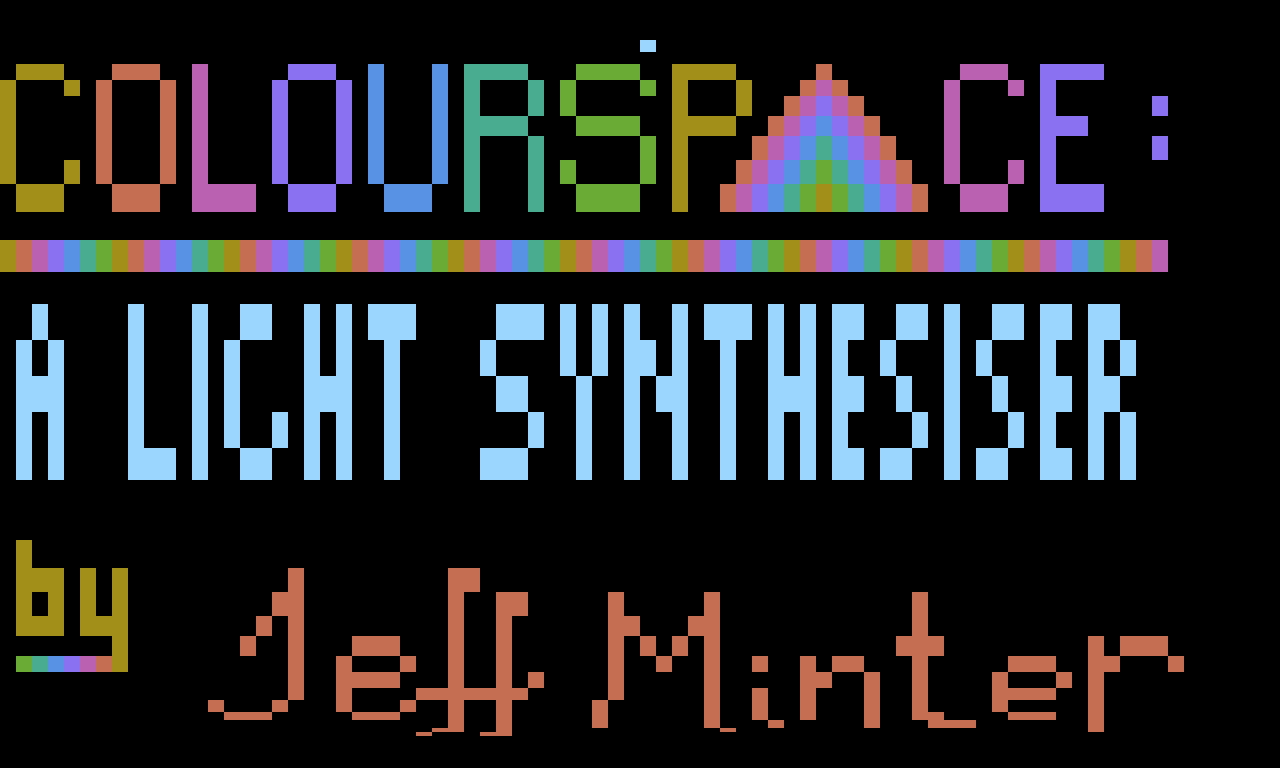
\includegraphics[width=12cm]{src/colorspace_painting/foregrounds/pixel_pattern_3.png}}%
    \end{adjustbox}
\caption{'Curved Colourspace 2' Display Mode}
\end{figure}

%
% CURVE + HARD REFLECT
%
\clearpage
\begin{minipage}[b]{0.31\linewidth}
  \begin{figure}[H]
    {
      \setlength{\tabcolsep}{3.0pt}
      \setlength\cmidrulewidth{\heavyrulewidth} % Make cmidrule = 
      \begin{adjustbox}{height=8.5cm}

        \begin{tabular}{lll}
          \toprule
          Bytes       & Description                                                         \\
          \midrule
          \icode{\$70}  & Draw 8 Blank Lines  \\
\icode{\$70}  & Draw 8 Blank Lines  \\
\icode{\$46} \icode{\$A150} & Read 40 bytes from: \icode{\$50A1} \\
\icode{\$90}  & Draw 2 Blank Lines  \\
\icode{\$4F} \icode{\$0070} & Read 40 bytes from: \icode{\$7000} \\
\icode{\$4F} \icode{\$2870} & Read 40 bytes from: \icode{\$7028} \\
\icode{\$4F} \icode{\$5070} & Read 40 bytes from: \icode{\$7050} \\
\icode{\$4F} \icode{\$5070} & Read 40 bytes from: \icode{\$7050} \\
\icode{\$4F} \icode{\$7870} & Read 40 bytes from: \icode{\$7078} \\
\icode{\$4F} \icode{\$7870} & Read 40 bytes from: \icode{\$7078} \\
\icode{\$4F} \icode{\$A070} & Read 40 bytes from: \icode{\$70A0} \\
\icode{\$4F} \icode{\$A070} & Read 40 bytes from: \icode{\$70A0} \\
\icode{\$4F} \icode{\$A070} & Read 40 bytes from: \icode{\$70A0} \\
\icode{\$4F} \icode{\$C870} & Read 40 bytes from: \icode{\$70C8} \\
\icode{\$4F} \icode{\$C870} & Read 40 bytes from: \icode{\$70C8} \\
\icode{\$4F} \icode{\$C870} & Read 40 bytes from: \icode{\$70C8} \\
\icode{\$4F} \icode{\$F070} & Read 40 bytes from: \icode{\$70F0} \\
\icode{\$4F} \icode{\$F070} & Read 40 bytes from: \icode{\$70F0} \\
\icode{\$4F} \icode{\$F070} & Read 40 bytes from: \icode{\$70F0} \\
\icode{\$4F} \icode{\$F070} & Read 40 bytes from: \icode{\$70F0} \\
\icode{\$4F} \icode{\$1871} & Read 40 bytes from: \icode{\$7118} \\
\icode{\$4F} \icode{\$1871} & Read 40 bytes from: \icode{\$7118} \\
\icode{\$4F} \icode{\$1871} & Read 40 bytes from: \icode{\$7118} \\
\icode{\$4F} \icode{\$1871} & Read 40 bytes from: \icode{\$7118} \\
\icode{\$4F} \icode{\$4071} & Read 40 bytes from: \icode{\$7140} \\
\icode{\$4F} \icode{\$4071} & Read 40 bytes from: \icode{\$7140} \\
\icode{\$4F} \icode{\$4071} & Read 40 bytes from: \icode{\$7140} \\
\icode{\$4F} \icode{\$4071} & Read 40 bytes from: \icode{\$7140} \\
\icode{\$4F} \icode{\$4071} & Read 40 bytes from: \icode{\$7140} \\
\icode{\$4F} \icode{\$6871} & Read 40 bytes from: \icode{\$7168} \\
\icode{\$4F} \icode{\$6871} & Read 40 bytes from: \icode{\$7168} \\
\icode{\$4F} \icode{\$6871} & Read 40 bytes from: \icode{\$7168} \\
\icode{\$4F} \icode{\$6871} & Read 40 bytes from: \icode{\$7168} \\
\icode{\$4F} \icode{\$6871} & Read 40 bytes from: \icode{\$7168} \\
\icode{\$4F} \icode{\$9071} & Read 40 bytes from: \icode{\$7190} \\
\icode{\$4F} \icode{\$9071} & Read 40 bytes from: \icode{\$7190} \\
\icode{\$4F} \icode{\$9071} & Read 40 bytes from: \icode{\$7190} \\
\icode{\$4F} \icode{\$9071} & Read 40 bytes from: \icode{\$7190} \\
\icode{\$4F} \icode{\$9071} & Read 40 bytes from: \icode{\$7190} \\
\icode{\$4F} \icode{\$9071} & Read 40 bytes from: \icode{\$7190} \\
\icode{\$4F} \icode{\$B871} & Read 40 bytes from: \icode{\$71B8} \\
\icode{\$4F} \icode{\$B871} & Read 40 bytes from: \icode{\$71B8} \\
\icode{\$4F} \icode{\$B871} & Read 40 bytes from: \icode{\$71B8} \\
\icode{\$4F} \icode{\$B871} & Read 40 bytes from: \icode{\$71B8} \\
\icode{\$4F} \icode{\$B871} & Read 40 bytes from: \icode{\$71B8} \\
\icode{\$4F} \icode{\$B871} & Read 40 bytes from: \icode{\$71B8} \\
\icode{\$4F} \icode{\$E071} & Read 40 bytes from: \icode{\$71E0} \\
\icode{\$4F} \icode{\$E071} & Read 40 bytes from: \icode{\$71E0} \\
\icode{\$4F} \icode{\$E071} & Read 40 bytes from: \icode{\$71E0} \\
\icode{\$4F} \icode{\$E071} & Read 40 bytes from: \icode{\$71E0} \\
\icode{\$4F} \icode{\$E071} & Read 40 bytes from: \icode{\$71E0} \\
\icode{\$4F} \icode{\$E071} & Read 40 bytes from: \icode{\$71E0} \\
\icode{\$4F} \icode{\$E071} & Read 40 bytes from: \icode{\$71E0} \\
\icode{\$4F} \icode{\$0872} & Read 40 bytes from: \icode{\$7208} \\
\icode{\$4F} \icode{\$0872} & Read 40 bytes from: \icode{\$7208} \\
\icode{\$4F} \icode{\$0872} & Read 40 bytes from: \icode{\$7208} \\
\icode{\$4F} \icode{\$0872} & Read 40 bytes from: \icode{\$7208} \\
\icode{\$4F} \icode{\$0872} & Read 40 bytes from: \icode{\$7208} \\
\icode{\$4F} \icode{\$0872} & Read 40 bytes from: \icode{\$7208} \\
\icode{\$4F} \icode{\$0872} & Read 40 bytes from: \icode{\$7208} \\
\icode{\$4F} \icode{\$3072} & Read 40 bytes from: \icode{\$7230} \\
\bottomrule

        \end{tabular}

      \end{adjustbox}

    }\caption*{Display List Entries: 1-61}
  \end{figure}
\end{minipage}
\hspace{0.1cm}
\begin{minipage}[b]{0.31\linewidth}
  \begin{figure}[H]
    {
      \setlength{\tabcolsep}{3.0pt}
      \setlength\cmidrulewidth{\heavyrulewidth} % Make cmidrule = 
      \begin{adjustbox}{height=8.5cm}

        \begin{tabular}{lll}
          \toprule
          Bytes       & Description                                                         \\
          \midrule
          \icode{\$4F} \icode{\$3072} & Read 40 bytes from: \icode{\$7230} \\
\icode{\$4F} \icode{\$3072} & Read 40 bytes from: \icode{\$7230} \\
\icode{\$4F} \icode{\$3072} & Read 40 bytes from: \icode{\$7230} \\
\icode{\$4F} \icode{\$3072} & Read 40 bytes from: \icode{\$7230} \\
\icode{\$4F} \icode{\$3072} & Read 40 bytes from: \icode{\$7230} \\
\icode{\$4F} \icode{\$3072} & Read 40 bytes from: \icode{\$7230} \\
\icode{\$4F} \icode{\$3072} & Read 40 bytes from: \icode{\$7230} \\
\icode{\$4F} \icode{\$5872} & Read 40 bytes from: \icode{\$7258} \\
\icode{\$4F} \icode{\$5872} & Read 40 bytes from: \icode{\$7258} \\
\icode{\$4F} \icode{\$5872} & Read 40 bytes from: \icode{\$7258} \\
\icode{\$4F} \icode{\$5872} & Read 40 bytes from: \icode{\$7258} \\
\icode{\$4F} \icode{\$5872} & Read 40 bytes from: \icode{\$7258} \\
\icode{\$4F} \icode{\$5872} & Read 40 bytes from: \icode{\$7258} \\
\icode{\$4F} \icode{\$5872} & Read 40 bytes from: \icode{\$7258} \\
\icode{\$4F} \icode{\$5872} & Read 40 bytes from: \icode{\$7258} \\
\icode{\$4F} \icode{\$8072} & Read 40 bytes from: \icode{\$7280} \\
\icode{\$4F} \icode{\$8072} & Read 40 bytes from: \icode{\$7280} \\
\icode{\$4F} \icode{\$8072} & Read 40 bytes from: \icode{\$7280} \\
\icode{\$4F} \icode{\$8072} & Read 40 bytes from: \icode{\$7280} \\
\icode{\$4F} \icode{\$8072} & Read 40 bytes from: \icode{\$7280} \\
\icode{\$4F} \icode{\$8072} & Read 40 bytes from: \icode{\$7280} \\
\icode{\$4F} \icode{\$8072} & Read 40 bytes from: \icode{\$7280} \\
\icode{\$4F} \icode{\$8072} & Read 40 bytes from: \icode{\$7280} \\
\icode{\$4F} \icode{\$8072} & Read 40 bytes from: \icode{\$7280} \\
\icode{\$4F} \icode{\$A872} & Read 40 bytes from: \icode{\$72A8} \\
\icode{\$4F} \icode{\$A872} & Read 40 bytes from: \icode{\$72A8} \\
\icode{\$4F} \icode{\$A872} & Read 40 bytes from: \icode{\$72A8} \\
\icode{\$4F} \icode{\$A872} & Read 40 bytes from: \icode{\$72A8} \\
\icode{\$4F} \icode{\$A872} & Read 40 bytes from: \icode{\$72A8} \\
\icode{\$4F} \icode{\$A872} & Read 40 bytes from: \icode{\$72A8} \\
\icode{\$4F} \icode{\$A872} & Read 40 bytes from: \icode{\$72A8} \\
\icode{\$4F} \icode{\$A872} & Read 40 bytes from: \icode{\$72A8} \\
\icode{\$4F} \icode{\$A872} & Read 40 bytes from: \icode{\$72A8} \\
\icode{\$4F} \icode{\$D072} & Read 40 bytes from: \icode{\$72D0} \\
\icode{\$4F} \icode{\$D072} & Read 40 bytes from: \icode{\$72D0} \\
\icode{\$4F} \icode{\$D072} & Read 40 bytes from: \icode{\$72D0} \\
\icode{\$4F} \icode{\$D072} & Read 40 bytes from: \icode{\$72D0} \\
\icode{\$4F} \icode{\$D072} & Read 40 bytes from: \icode{\$72D0} \\
\icode{\$4F} \icode{\$D072} & Read 40 bytes from: \icode{\$72D0} \\
\icode{\$4F} \icode{\$D072} & Read 40 bytes from: \icode{\$72D0} \\
\icode{\$4F} \icode{\$D072} & Read 40 bytes from: \icode{\$72D0} \\
\icode{\$4F} \icode{\$D072} & Read 40 bytes from: \icode{\$72D0} \\
\icode{\$4F} \icode{\$A872} & Read 40 bytes from: \icode{\$72A8} \\
\icode{\$4F} \icode{\$A872} & Read 40 bytes from: \icode{\$72A8} \\
\icode{\$4F} \icode{\$A872} & Read 40 bytes from: \icode{\$72A8} \\
\icode{\$4F} \icode{\$A872} & Read 40 bytes from: \icode{\$72A8} \\
\icode{\$4F} \icode{\$A872} & Read 40 bytes from: \icode{\$72A8} \\
\icode{\$4F} \icode{\$A872} & Read 40 bytes from: \icode{\$72A8} \\
\icode{\$4F} \icode{\$A872} & Read 40 bytes from: \icode{\$72A8} \\
\icode{\$4F} \icode{\$A872} & Read 40 bytes from: \icode{\$72A8} \\
\icode{\$4F} \icode{\$A872} & Read 40 bytes from: \icode{\$72A8} \\
\icode{\$4F} \icode{\$8072} & Read 40 bytes from: \icode{\$7280} \\
\icode{\$4F} \icode{\$8072} & Read 40 bytes from: \icode{\$7280} \\
\icode{\$4F} \icode{\$8072} & Read 40 bytes from: \icode{\$7280} \\
\icode{\$4F} \icode{\$8072} & Read 40 bytes from: \icode{\$7280} \\
\icode{\$4F} \icode{\$8072} & Read 40 bytes from: \icode{\$7280} \\
\icode{\$4F} \icode{\$8072} & Read 40 bytes from: \icode{\$7280} \\
\icode{\$4F} \icode{\$8072} & Read 40 bytes from: \icode{\$7280} \\
\icode{\$4F} \icode{\$8072} & Read 40 bytes from: \icode{\$7280} \\
\icode{\$4F} \icode{\$5872} & Read 40 bytes from: \icode{\$7258} \\
\icode{\$4F} \icode{\$5872} & Read 40 bytes from: \icode{\$7258} \\
\bottomrule
%
        \end{tabular}

      \end{adjustbox}

    }\caption*{Display List Entries: 62-122}
  \end{figure}
\end{minipage}
\hspace{0.1cm}
\begin{minipage}[b]{0.31\linewidth}
  \begin{figure}[H]
    {
      \setlength{\tabcolsep}{3.0pt}
      \setlength\cmidrulewidth{\heavyrulewidth} % Make cmidrule = 
      \begin{adjustbox}{height=8.5cm}

        \begin{tabular}{lll}
          \toprule
          Bytes       & Description                                                         \\
          \midrule
          \icode{\$4F} \icode{\$5872} & Read 40 bytes from: \icode{\$7258} \\
\icode{\$4F} \icode{\$5872} & Read 40 bytes from: \icode{\$7258} \\
\icode{\$4F} \icode{\$5872} & Read 40 bytes from: \icode{\$7258} \\
\icode{\$4F} \icode{\$5872} & Read 40 bytes from: \icode{\$7258} \\
\icode{\$4F} \icode{\$5872} & Read 40 bytes from: \icode{\$7258} \\
\icode{\$4F} \icode{\$5872} & Read 40 bytes from: \icode{\$7258} \\
\icode{\$4F} \icode{\$3072} & Read 40 bytes from: \icode{\$7230} \\
\icode{\$4F} \icode{\$3072} & Read 40 bytes from: \icode{\$7230} \\
\icode{\$4F} \icode{\$3072} & Read 40 bytes from: \icode{\$7230} \\
\icode{\$4F} \icode{\$3072} & Read 40 bytes from: \icode{\$7230} \\
\icode{\$4F} \icode{\$3072} & Read 40 bytes from: \icode{\$7230} \\
\icode{\$4F} \icode{\$3072} & Read 40 bytes from: \icode{\$7230} \\
\icode{\$4F} \icode{\$3072} & Read 40 bytes from: \icode{\$7230} \\
\icode{\$4F} \icode{\$0872} & Read 40 bytes from: \icode{\$7208} \\
\icode{\$4F} \icode{\$0872} & Read 40 bytes from: \icode{\$7208} \\
\icode{\$4F} \icode{\$0872} & Read 40 bytes from: \icode{\$7208} \\
\icode{\$4F} \icode{\$0872} & Read 40 bytes from: \icode{\$7208} \\
\icode{\$4F} \icode{\$0872} & Read 40 bytes from: \icode{\$7208} \\
\icode{\$4F} \icode{\$0872} & Read 40 bytes from: \icode{\$7208} \\
\icode{\$4F} \icode{\$0872} & Read 40 bytes from: \icode{\$7208} \\
\icode{\$4F} \icode{\$E071} & Read 40 bytes from: \icode{\$71E0} \\
\icode{\$4F} \icode{\$E071} & Read 40 bytes from: \icode{\$71E0} \\
\icode{\$4F} \icode{\$E071} & Read 40 bytes from: \icode{\$71E0} \\
\icode{\$4F} \icode{\$E071} & Read 40 bytes from: \icode{\$71E0} \\
\icode{\$4F} \icode{\$E071} & Read 40 bytes from: \icode{\$71E0} \\
\icode{\$4F} \icode{\$E071} & Read 40 bytes from: \icode{\$71E0} \\
\icode{\$4F} \icode{\$B871} & Read 40 bytes from: \icode{\$71B8} \\
\icode{\$4F} \icode{\$B871} & Read 40 bytes from: \icode{\$71B8} \\
\icode{\$4F} \icode{\$B871} & Read 40 bytes from: \icode{\$71B8} \\
\icode{\$4F} \icode{\$B871} & Read 40 bytes from: \icode{\$71B8} \\
\icode{\$4F} \icode{\$B871} & Read 40 bytes from: \icode{\$71B8} \\
\icode{\$4F} \icode{\$B871} & Read 40 bytes from: \icode{\$71B8} \\
\icode{\$4F} \icode{\$9071} & Read 40 bytes from: \icode{\$7190} \\
\icode{\$4F} \icode{\$9071} & Read 40 bytes from: \icode{\$7190} \\
\icode{\$4F} \icode{\$9071} & Read 40 bytes from: \icode{\$7190} \\
\icode{\$4F} \icode{\$9071} & Read 40 bytes from: \icode{\$7190} \\
\icode{\$4F} \icode{\$9071} & Read 40 bytes from: \icode{\$7190} \\
\icode{\$4F} \icode{\$6871} & Read 40 bytes from: \icode{\$7168} \\
\icode{\$4F} \icode{\$6871} & Read 40 bytes from: \icode{\$7168} \\
\icode{\$4F} \icode{\$6871} & Read 40 bytes from: \icode{\$7168} \\
\icode{\$4F} \icode{\$6871} & Read 40 bytes from: \icode{\$7168} \\
\icode{\$4F} \icode{\$6871} & Read 40 bytes from: \icode{\$7168} \\
\icode{\$4F} \icode{\$4071} & Read 40 bytes from: \icode{\$7140} \\
\icode{\$4F} \icode{\$4071} & Read 40 bytes from: \icode{\$7140} \\
\icode{\$4F} \icode{\$4071} & Read 40 bytes from: \icode{\$7140} \\
\icode{\$4F} \icode{\$4071} & Read 40 bytes from: \icode{\$7140} \\
\icode{\$4F} \icode{\$1871} & Read 40 bytes from: \icode{\$7118} \\
\icode{\$4F} \icode{\$1871} & Read 40 bytes from: \icode{\$7118} \\
\icode{\$4F} \icode{\$1871} & Read 40 bytes from: \icode{\$7118} \\
\icode{\$4F} \icode{\$1871} & Read 40 bytes from: \icode{\$7118} \\
\icode{\$4F} \icode{\$F070} & Read 40 bytes from: \icode{\$70F0} \\
\icode{\$4F} \icode{\$F070} & Read 40 bytes from: \icode{\$70F0} \\
\icode{\$4F} \icode{\$F070} & Read 40 bytes from: \icode{\$70F0} \\
\icode{\$4F} \icode{\$C870} & Read 40 bytes from: \icode{\$70C8} \\
\icode{\$4F} \icode{\$C870} & Read 40 bytes from: \icode{\$70C8} \\
\icode{\$4F} \icode{\$C870} & Read 40 bytes from: \icode{\$70C8} \\
\icode{\$4F} \icode{\$A070} & Read 40 bytes from: \icode{\$70A0} \\
\icode{\$4F} \icode{\$A070} & Read 40 bytes from: \icode{\$70A0} \\
\icode{\$4F} \icode{\$7870} & Read 40 bytes from: \icode{\$7078} \\
\icode{\$4F} \icode{\$7870} & Read 40 bytes from: \icode{\$7078} \\
\icode{\$4F} \icode{\$5070} & Read 40 bytes from: \icode{\$7050} \\
\icode{\$4F} \icode{\$2870} & Read 40 bytes from: \icode{\$7028} \\
\bottomrule
%
        \end{tabular}

      \end{adjustbox}

    }\caption*{Display List Entries: 123-182}
  \end{figure}
\end{minipage}

\clearpage
\begin{figure}[H]
    \centering
    \begin{adjustbox}{width=12cm,center}
      \frame{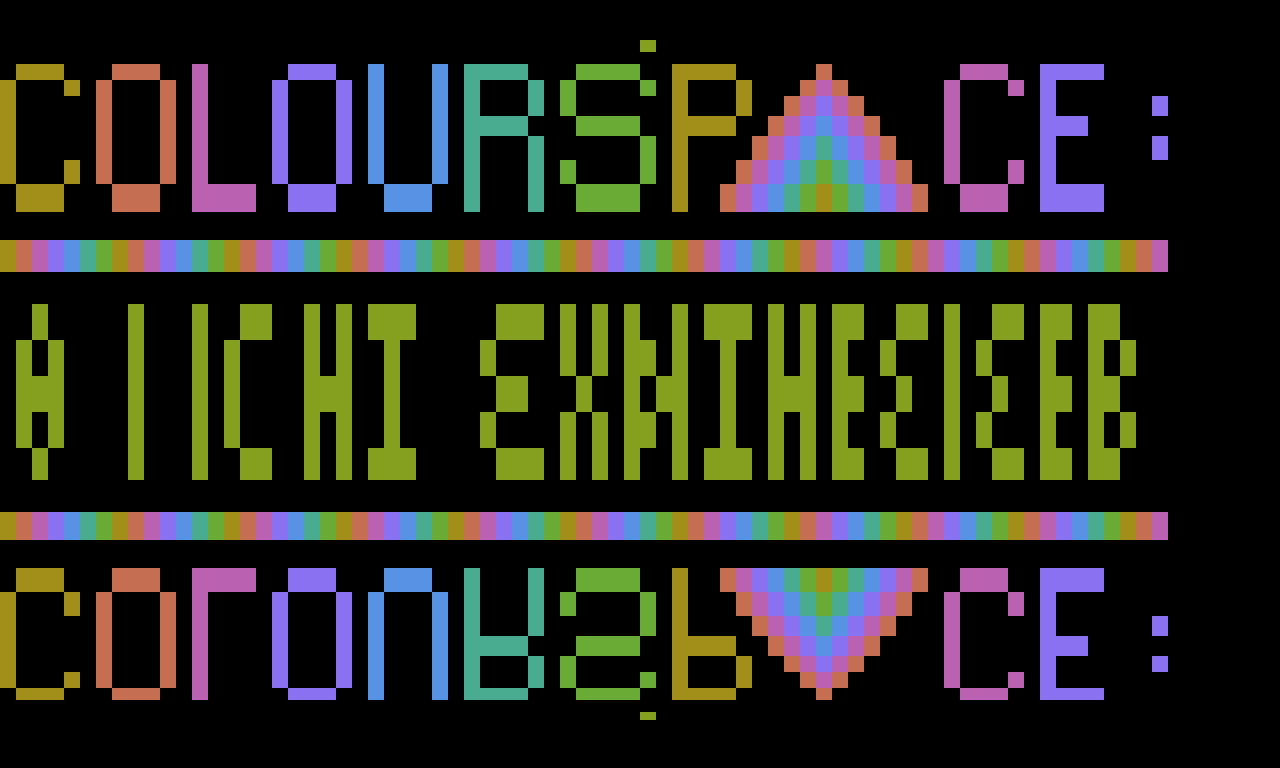
\includegraphics[width=12cm]{src/colorspace_painting/foregrounds/pixel_pattern_4.png}}%
    \end{adjustbox}
\caption{'Curved + Hard Reflect' Display Mode}
\end{figure}

%
% HOOPY 4x CURVEYREFLEX
%
\clearpage
\begin{minipage}[b]{0.31\linewidth}
  \begin{figure}[H]
    {
      \setlength{\tabcolsep}{3.0pt}
      \setlength\cmidrulewidth{\heavyrulewidth} % Make cmidrule = 
      \begin{adjustbox}{height=8.5cm}

        \begin{tabular}{lll}
          \toprule
          Bytes       & Description                                                         \\
          \midrule
          \icode{\$70}  & Draw 8 Blank Lines  \\
\icode{\$70}  & Draw 8 Blank Lines  \\
\icode{\$46} \icode{\$B550} & Read 40 bytes from: \icode{\$50B5} \\
\icode{\$90}  & Draw 2 Blank Lines  \\
\icode{\$4F} \icode{\$0070} & Read 40 bytes from: \icode{\$7000} \\
\icode{\$4F} \icode{\$2870} & Read 40 bytes from: \icode{\$7028} \\
\icode{\$4F} \icode{\$2870} & Read 40 bytes from: \icode{\$7028} \\
\icode{\$4F} \icode{\$5070} & Read 40 bytes from: \icode{\$7050} \\
\icode{\$4F} \icode{\$5070} & Read 40 bytes from: \icode{\$7050} \\
\icode{\$4F} \icode{\$5070} & Read 40 bytes from: \icode{\$7050} \\
\icode{\$4F} \icode{\$7870} & Read 40 bytes from: \icode{\$7078} \\
\icode{\$4F} \icode{\$7870} & Read 40 bytes from: \icode{\$7078} \\
\icode{\$4F} \icode{\$7870} & Read 40 bytes from: \icode{\$7078} \\
\icode{\$4F} \icode{\$7870} & Read 40 bytes from: \icode{\$7078} \\
\icode{\$4F} \icode{\$A070} & Read 40 bytes from: \icode{\$70A0} \\
\icode{\$4F} \icode{\$A070} & Read 40 bytes from: \icode{\$70A0} \\
\icode{\$4F} \icode{\$A070} & Read 40 bytes from: \icode{\$70A0} \\
\icode{\$4F} \icode{\$A070} & Read 40 bytes from: \icode{\$70A0} \\
\icode{\$4F} \icode{\$A070} & Read 40 bytes from: \icode{\$70A0} \\
\icode{\$4F} \icode{\$C870} & Read 40 bytes from: \icode{\$70C8} \\
\icode{\$4F} \icode{\$C870} & Read 40 bytes from: \icode{\$70C8} \\
\icode{\$4F} \icode{\$C870} & Read 40 bytes from: \icode{\$70C8} \\
\icode{\$4F} \icode{\$C870} & Read 40 bytes from: \icode{\$70C8} \\
\icode{\$4F} \icode{\$C870} & Read 40 bytes from: \icode{\$70C8} \\
\icode{\$4F} \icode{\$C870} & Read 40 bytes from: \icode{\$70C8} \\
\icode{\$4F} \icode{\$F070} & Read 40 bytes from: \icode{\$70F0} \\
\icode{\$4F} \icode{\$F070} & Read 40 bytes from: \icode{\$70F0} \\
\icode{\$4F} \icode{\$F070} & Read 40 bytes from: \icode{\$70F0} \\
\icode{\$4F} \icode{\$F070} & Read 40 bytes from: \icode{\$70F0} \\
\icode{\$4F} \icode{\$F070} & Read 40 bytes from: \icode{\$70F0} \\
\icode{\$4F} \icode{\$F070} & Read 40 bytes from: \icode{\$70F0} \\
\icode{\$4F} \icode{\$F070} & Read 40 bytes from: \icode{\$70F0} \\
\icode{\$4F} \icode{\$1871} & Read 40 bytes from: \icode{\$7118} \\
\icode{\$4F} \icode{\$1871} & Read 40 bytes from: \icode{\$7118} \\
\icode{\$4F} \icode{\$1871} & Read 40 bytes from: \icode{\$7118} \\
\icode{\$4F} \icode{\$1871} & Read 40 bytes from: \icode{\$7118} \\
\icode{\$4F} \icode{\$1871} & Read 40 bytes from: \icode{\$7118} \\
\icode{\$4F} \icode{\$1871} & Read 40 bytes from: \icode{\$7118} \\
\icode{\$4F} \icode{\$1871} & Read 40 bytes from: \icode{\$7118} \\
\icode{\$4F} \icode{\$1871} & Read 40 bytes from: \icode{\$7118} \\
\icode{\$4F} \icode{\$4071} & Read 40 bytes from: \icode{\$7140} \\
\icode{\$4F} \icode{\$4071} & Read 40 bytes from: \icode{\$7140} \\
\icode{\$4F} \icode{\$4071} & Read 40 bytes from: \icode{\$7140} \\
\icode{\$4F} \icode{\$4071} & Read 40 bytes from: \icode{\$7140} \\
\icode{\$4F} \icode{\$4071} & Read 40 bytes from: \icode{\$7140} \\
\icode{\$4F} \icode{\$4071} & Read 40 bytes from: \icode{\$7140} \\
\icode{\$4F} \icode{\$4071} & Read 40 bytes from: \icode{\$7140} \\
\icode{\$4F} \icode{\$4071} & Read 40 bytes from: \icode{\$7140} \\
\icode{\$4F} \icode{\$4071} & Read 40 bytes from: \icode{\$7140} \\
\icode{\$4F} \icode{\$6871} & Read 40 bytes from: \icode{\$7168} \\
\icode{\$4F} \icode{\$6871} & Read 40 bytes from: \icode{\$7168} \\
\icode{\$4F} \icode{\$6871} & Read 40 bytes from: \icode{\$7168} \\
\icode{\$4F} \icode{\$6871} & Read 40 bytes from: \icode{\$7168} \\
\icode{\$4F} \icode{\$6871} & Read 40 bytes from: \icode{\$7168} \\
\icode{\$4F} \icode{\$6871} & Read 40 bytes from: \icode{\$7168} \\
\icode{\$4F} \icode{\$6871} & Read 40 bytes from: \icode{\$7168} \\
\icode{\$4F} \icode{\$6871} & Read 40 bytes from: \icode{\$7168} \\
\icode{\$4F} \icode{\$6871} & Read 40 bytes from: \icode{\$7168} \\
\icode{\$4F} \icode{\$4071} & Read 40 bytes from: \icode{\$7140} \\
\icode{\$4F} \icode{\$4071} & Read 40 bytes from: \icode{\$7140} \\
\icode{\$4F} \icode{\$4071} & Read 40 bytes from: \icode{\$7140} \\
\bottomrule

        \end{tabular}

      \end{adjustbox}

    }\caption*{Display List Entries: 1-61}
  \end{figure}
\end{minipage}
\hspace{0.1cm}
\begin{minipage}[b]{0.31\linewidth}
  \begin{figure}[H]
    {
      \setlength{\tabcolsep}{3.0pt}
      \setlength\cmidrulewidth{\heavyrulewidth} % Make cmidrule = 
      \begin{adjustbox}{height=8.5cm}

        \begin{tabular}{lll}
          \toprule
          Bytes       & Description                                                         \\
          \midrule
          \icode{\$4F} \icode{\$4071} & Read 40 bytes from: \icode{\$7140} \\
\icode{\$4F} \icode{\$4071} & Read 40 bytes from: \icode{\$7140} \\
\icode{\$4F} \icode{\$4071} & Read 40 bytes from: \icode{\$7140} \\
\icode{\$4F} \icode{\$4071} & Read 40 bytes from: \icode{\$7140} \\
\icode{\$4F} \icode{\$4071} & Read 40 bytes from: \icode{\$7140} \\
\icode{\$4F} \icode{\$1871} & Read 40 bytes from: \icode{\$7118} \\
\icode{\$4F} \icode{\$1871} & Read 40 bytes from: \icode{\$7118} \\
\icode{\$4F} \icode{\$1871} & Read 40 bytes from: \icode{\$7118} \\
\icode{\$4F} \icode{\$1871} & Read 40 bytes from: \icode{\$7118} \\
\icode{\$4F} \icode{\$1871} & Read 40 bytes from: \icode{\$7118} \\
\icode{\$4F} \icode{\$1871} & Read 40 bytes from: \icode{\$7118} \\
\icode{\$4F} \icode{\$1871} & Read 40 bytes from: \icode{\$7118} \\
\icode{\$4F} \icode{\$F070} & Read 40 bytes from: \icode{\$70F0} \\
\icode{\$4F} \icode{\$F070} & Read 40 bytes from: \icode{\$70F0} \\
\icode{\$4F} \icode{\$F070} & Read 40 bytes from: \icode{\$70F0} \\
\icode{\$4F} \icode{\$F070} & Read 40 bytes from: \icode{\$70F0} \\
\icode{\$4F} \icode{\$F070} & Read 40 bytes from: \icode{\$70F0} \\
\icode{\$4F} \icode{\$F070} & Read 40 bytes from: \icode{\$70F0} \\
\icode{\$4F} \icode{\$C870} & Read 40 bytes from: \icode{\$70C8} \\
\icode{\$4F} \icode{\$C870} & Read 40 bytes from: \icode{\$70C8} \\
\icode{\$4F} \icode{\$C870} & Read 40 bytes from: \icode{\$70C8} \\
\icode{\$4F} \icode{\$C870} & Read 40 bytes from: \icode{\$70C8} \\
\icode{\$4F} \icode{\$C870} & Read 40 bytes from: \icode{\$70C8} \\
\icode{\$4F} \icode{\$A070} & Read 40 bytes from: \icode{\$70A0} \\
\icode{\$4F} \icode{\$A070} & Read 40 bytes from: \icode{\$70A0} \\
\icode{\$4F} \icode{\$A070} & Read 40 bytes from: \icode{\$70A0} \\
\icode{\$4F} \icode{\$A070} & Read 40 bytes from: \icode{\$70A0} \\
\icode{\$4F} \icode{\$7870} & Read 40 bytes from: \icode{\$7078} \\
\icode{\$4F} \icode{\$7870} & Read 40 bytes from: \icode{\$7078} \\
\icode{\$4F} \icode{\$7870} & Read 40 bytes from: \icode{\$7078} \\
\icode{\$4F} \icode{\$5070} & Read 40 bytes from: \icode{\$7050} \\
\icode{\$4F} \icode{\$5070} & Read 40 bytes from: \icode{\$7050} \\
\icode{\$4F} \icode{\$2870} & Read 40 bytes from: \icode{\$7028} \\
\icode{\$4F} \icode{\$0070} & Read 40 bytes from: \icode{\$7000} \\
\icode{\$4F} \icode{\$2870} & Read 40 bytes from: \icode{\$7028} \\
\icode{\$4F} \icode{\$2870} & Read 40 bytes from: \icode{\$7028} \\
\icode{\$4F} \icode{\$5070} & Read 40 bytes from: \icode{\$7050} \\
\icode{\$4F} \icode{\$5070} & Read 40 bytes from: \icode{\$7050} \\
\icode{\$4F} \icode{\$5070} & Read 40 bytes from: \icode{\$7050} \\
\icode{\$4F} \icode{\$7870} & Read 40 bytes from: \icode{\$7078} \\
\icode{\$4F} \icode{\$7870} & Read 40 bytes from: \icode{\$7078} \\
\icode{\$4F} \icode{\$7870} & Read 40 bytes from: \icode{\$7078} \\
\icode{\$4F} \icode{\$7870} & Read 40 bytes from: \icode{\$7078} \\
\icode{\$4F} \icode{\$A070} & Read 40 bytes from: \icode{\$70A0} \\
\icode{\$4F} \icode{\$A070} & Read 40 bytes from: \icode{\$70A0} \\
\icode{\$4F} \icode{\$A070} & Read 40 bytes from: \icode{\$70A0} \\
\icode{\$4F} \icode{\$A070} & Read 40 bytes from: \icode{\$70A0} \\
\icode{\$4F} \icode{\$A070} & Read 40 bytes from: \icode{\$70A0} \\
\icode{\$4F} \icode{\$C870} & Read 40 bytes from: \icode{\$70C8} \\
\icode{\$4F} \icode{\$C870} & Read 40 bytes from: \icode{\$70C8} \\
\icode{\$4F} \icode{\$C870} & Read 40 bytes from: \icode{\$70C8} \\
\icode{\$4F} \icode{\$C870} & Read 40 bytes from: \icode{\$70C8} \\
\icode{\$4F} \icode{\$C870} & Read 40 bytes from: \icode{\$70C8} \\
\icode{\$4F} \icode{\$C870} & Read 40 bytes from: \icode{\$70C8} \\
\icode{\$4F} \icode{\$F070} & Read 40 bytes from: \icode{\$70F0} \\
\icode{\$4F} \icode{\$F070} & Read 40 bytes from: \icode{\$70F0} \\
\icode{\$4F} \icode{\$F070} & Read 40 bytes from: \icode{\$70F0} \\
\icode{\$4F} \icode{\$F070} & Read 40 bytes from: \icode{\$70F0} \\
\icode{\$4F} \icode{\$F070} & Read 40 bytes from: \icode{\$70F0} \\
\icode{\$4F} \icode{\$F070} & Read 40 bytes from: \icode{\$70F0} \\
\icode{\$4F} \icode{\$F070} & Read 40 bytes from: \icode{\$70F0} \\
\bottomrule
%
        \end{tabular}

      \end{adjustbox}

    }\caption*{Display List Entries: 62-122}
  \end{figure}
\end{minipage}
\hspace{0.1cm}
\begin{minipage}[b]{0.31\linewidth}
  \begin{figure}[H]
    {
      \setlength{\tabcolsep}{3.0pt}
      \setlength\cmidrulewidth{\heavyrulewidth} % Make cmidrule = 
      \begin{adjustbox}{height=8.5cm}

        \begin{tabular}{lll}
          \toprule
          Bytes       & Description                                                         \\
          \midrule
          \icode{\$4F} \icode{\$1871} & Read 40 bytes from: \icode{\$7118} \\
\icode{\$4F} \icode{\$1871} & Read 40 bytes from: \icode{\$7118} \\
\icode{\$4F} \icode{\$1871} & Read 40 bytes from: \icode{\$7118} \\
\icode{\$4F} \icode{\$1871} & Read 40 bytes from: \icode{\$7118} \\
\icode{\$4F} \icode{\$1871} & Read 40 bytes from: \icode{\$7118} \\
\icode{\$4F} \icode{\$1871} & Read 40 bytes from: \icode{\$7118} \\
\icode{\$4F} \icode{\$1871} & Read 40 bytes from: \icode{\$7118} \\
\icode{\$4F} \icode{\$1871} & Read 40 bytes from: \icode{\$7118} \\
\icode{\$4F} \icode{\$4071} & Read 40 bytes from: \icode{\$7140} \\
\icode{\$4F} \icode{\$4071} & Read 40 bytes from: \icode{\$7140} \\
\icode{\$4F} \icode{\$4071} & Read 40 bytes from: \icode{\$7140} \\
\icode{\$4F} \icode{\$4071} & Read 40 bytes from: \icode{\$7140} \\
\icode{\$4F} \icode{\$4071} & Read 40 bytes from: \icode{\$7140} \\
\icode{\$4F} \icode{\$4071} & Read 40 bytes from: \icode{\$7140} \\
\icode{\$4F} \icode{\$4071} & Read 40 bytes from: \icode{\$7140} \\
\icode{\$4F} \icode{\$4071} & Read 40 bytes from: \icode{\$7140} \\
\icode{\$4F} \icode{\$4071} & Read 40 bytes from: \icode{\$7140} \\
\icode{\$4F} \icode{\$6871} & Read 40 bytes from: \icode{\$7168} \\
\icode{\$4F} \icode{\$6871} & Read 40 bytes from: \icode{\$7168} \\
\icode{\$4F} \icode{\$6871} & Read 40 bytes from: \icode{\$7168} \\
\icode{\$4F} \icode{\$6871} & Read 40 bytes from: \icode{\$7168} \\
\icode{\$4F} \icode{\$6871} & Read 40 bytes from: \icode{\$7168} \\
\icode{\$4F} \icode{\$6871} & Read 40 bytes from: \icode{\$7168} \\
\icode{\$4F} \icode{\$6871} & Read 40 bytes from: \icode{\$7168} \\
\icode{\$4F} \icode{\$6871} & Read 40 bytes from: \icode{\$7168} \\
\icode{\$4F} \icode{\$6871} & Read 40 bytes from: \icode{\$7168} \\
\icode{\$4F} \icode{\$4071} & Read 40 bytes from: \icode{\$7140} \\
\icode{\$4F} \icode{\$4071} & Read 40 bytes from: \icode{\$7140} \\
\icode{\$4F} \icode{\$4071} & Read 40 bytes from: \icode{\$7140} \\
\icode{\$4F} \icode{\$4071} & Read 40 bytes from: \icode{\$7140} \\
\icode{\$4F} \icode{\$4071} & Read 40 bytes from: \icode{\$7140} \\
\icode{\$4F} \icode{\$4071} & Read 40 bytes from: \icode{\$7140} \\
\icode{\$4F} \icode{\$4071} & Read 40 bytes from: \icode{\$7140} \\
\icode{\$4F} \icode{\$4071} & Read 40 bytes from: \icode{\$7140} \\
\icode{\$4F} \icode{\$1871} & Read 40 bytes from: \icode{\$7118} \\
\icode{\$4F} \icode{\$1871} & Read 40 bytes from: \icode{\$7118} \\
\icode{\$4F} \icode{\$1871} & Read 40 bytes from: \icode{\$7118} \\
\icode{\$4F} \icode{\$1871} & Read 40 bytes from: \icode{\$7118} \\
\icode{\$4F} \icode{\$1871} & Read 40 bytes from: \icode{\$7118} \\
\icode{\$4F} \icode{\$1871} & Read 40 bytes from: \icode{\$7118} \\
\icode{\$4F} \icode{\$1871} & Read 40 bytes from: \icode{\$7118} \\
\icode{\$4F} \icode{\$F070} & Read 40 bytes from: \icode{\$70F0} \\
\icode{\$4F} \icode{\$F070} & Read 40 bytes from: \icode{\$70F0} \\
\icode{\$4F} \icode{\$F070} & Read 40 bytes from: \icode{\$70F0} \\
\icode{\$4F} \icode{\$F070} & Read 40 bytes from: \icode{\$70F0} \\
\icode{\$4F} \icode{\$F070} & Read 40 bytes from: \icode{\$70F0} \\
\icode{\$4F} \icode{\$F070} & Read 40 bytes from: \icode{\$70F0} \\
\icode{\$4F} \icode{\$C870} & Read 40 bytes from: \icode{\$70C8} \\
\icode{\$4F} \icode{\$C870} & Read 40 bytes from: \icode{\$70C8} \\
\icode{\$4F} \icode{\$C870} & Read 40 bytes from: \icode{\$70C8} \\
\icode{\$4F} \icode{\$C870} & Read 40 bytes from: \icode{\$70C8} \\
\icode{\$4F} \icode{\$C870} & Read 40 bytes from: \icode{\$70C8} \\
\icode{\$4F} \icode{\$A070} & Read 40 bytes from: \icode{\$70A0} \\
\icode{\$4F} \icode{\$A070} & Read 40 bytes from: \icode{\$70A0} \\
\icode{\$4F} \icode{\$A070} & Read 40 bytes from: \icode{\$70A0} \\
\icode{\$4F} \icode{\$A070} & Read 40 bytes from: \icode{\$70A0} \\
\icode{\$4F} \icode{\$7870} & Read 40 bytes from: \icode{\$7078} \\
\icode{\$4F} \icode{\$7870} & Read 40 bytes from: \icode{\$7078} \\
\icode{\$4F} \icode{\$7870} & Read 40 bytes from: \icode{\$7078} \\
\icode{\$4F} \icode{\$5070} & Read 40 bytes from: \icode{\$7050} \\
\icode{\$4F} \icode{\$5070} & Read 40 bytes from: \icode{\$7050} \\
\icode{\$4F} \icode{\$2870} & Read 40 bytes from: \icode{\$7028} \\
\bottomrule
%
        \end{tabular}

      \end{adjustbox}

    }\caption*{Display List Entries: 123-182}
  \end{figure}
\end{minipage}

\clearpage
\begin{figure}[H]
    \centering
    \begin{adjustbox}{width=12cm,center}
      \frame{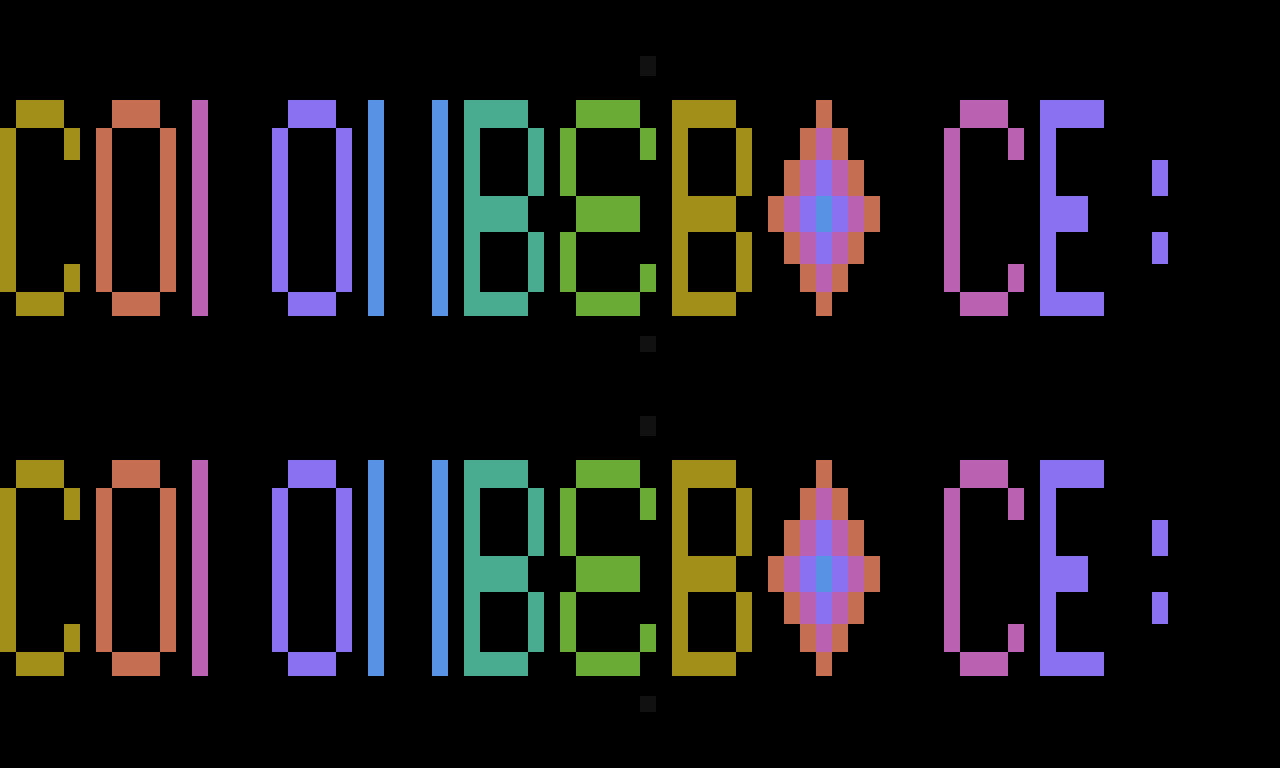
\includegraphics[width=12cm]{src/colorspace_painting/foregrounds/pixel_pattern_5.png}}%
    \end{adjustbox}
\caption{'Hoopy 4X CurvyReflex' Display Mode}
\end{figure}

%
% ZARJAX INTERLACE RES
%
\clearpage
\begin{minipage}[b]{0.31\linewidth}
  \begin{figure}[H]
    {
      \setlength{\tabcolsep}{3.0pt}
      \setlength\cmidrulewidth{\heavyrulewidth} % Make cmidrule = 
      \begin{adjustbox}{height=8.5cm}

        \begin{tabular}{lll}
          \toprule
          Bytes       & Description                                                         \\
          \midrule
          \icode{\$70}  & Draw 8 Blank Lines  \\
\icode{\$70}  & Draw 8 Blank Lines  \\
\icode{\$46} \icode{\$C950} & Read 40 bytes from: \icode{\$50C9} \\
\icode{\$90}  & Draw 2 Blank Lines  \\
\icode{\$4F} \icode{\$0070} & Read 40 bytes from: \icode{\$7000} \\
\icode{\$4F} \icode{\$E87D} & Read 40 bytes from: \icode{\$7DE8} \\
\icode{\$4F} \icode{\$2870} & Read 40 bytes from: \icode{\$7028} \\
\icode{\$4F} \icode{\$C07D} & Read 40 bytes from: \icode{\$7DC0} \\
\icode{\$4F} \icode{\$5070} & Read 40 bytes from: \icode{\$7050} \\
\icode{\$4F} \icode{\$987D} & Read 40 bytes from: \icode{\$7D98} \\
\icode{\$4F} \icode{\$7870} & Read 40 bytes from: \icode{\$7078} \\
\icode{\$4F} \icode{\$707D} & Read 40 bytes from: \icode{\$7D70} \\
\icode{\$4F} \icode{\$A070} & Read 40 bytes from: \icode{\$70A0} \\
\icode{\$4F} \icode{\$487D} & Read 40 bytes from: \icode{\$7D48} \\
\icode{\$4F} \icode{\$C870} & Read 40 bytes from: \icode{\$70C8} \\
\icode{\$4F} \icode{\$207D} & Read 40 bytes from: \icode{\$7D20} \\
\icode{\$4F} \icode{\$F070} & Read 40 bytes from: \icode{\$70F0} \\
\icode{\$4F} \icode{\$F87C} & Read 40 bytes from: \icode{\$7CF8} \\
\icode{\$4F} \icode{\$1871} & Read 40 bytes from: \icode{\$7118} \\
\icode{\$4F} \icode{\$D07C} & Read 40 bytes from: \icode{\$7CD0} \\
\icode{\$4F} \icode{\$4071} & Read 40 bytes from: \icode{\$7140} \\
\icode{\$4F} \icode{\$A87C} & Read 40 bytes from: \icode{\$7CA8} \\
\icode{\$4F} \icode{\$6871} & Read 40 bytes from: \icode{\$7168} \\
\icode{\$4F} \icode{\$807C} & Read 40 bytes from: \icode{\$7C80} \\
\icode{\$4F} \icode{\$9071} & Read 40 bytes from: \icode{\$7190} \\
\icode{\$4F} \icode{\$587C} & Read 40 bytes from: \icode{\$7C58} \\
\icode{\$4F} \icode{\$B871} & Read 40 bytes from: \icode{\$71B8} \\
\icode{\$4F} \icode{\$307C} & Read 40 bytes from: \icode{\$7C30} \\
\icode{\$4F} \icode{\$E071} & Read 40 bytes from: \icode{\$71E0} \\
\icode{\$4F} \icode{\$087C} & Read 40 bytes from: \icode{\$7C08} \\
\icode{\$4F} \icode{\$0872} & Read 40 bytes from: \icode{\$7208} \\
\icode{\$4F} \icode{\$E07B} & Read 40 bytes from: \icode{\$7BE0} \\
\icode{\$4F} \icode{\$3072} & Read 40 bytes from: \icode{\$7230} \\
\icode{\$4F} \icode{\$B87B} & Read 40 bytes from: \icode{\$7BB8} \\
\icode{\$4F} \icode{\$5872} & Read 40 bytes from: \icode{\$7258} \\
\icode{\$4F} \icode{\$907B} & Read 40 bytes from: \icode{\$7B90} \\
\icode{\$4F} \icode{\$8072} & Read 40 bytes from: \icode{\$7280} \\
\icode{\$4F} \icode{\$687B} & Read 40 bytes from: \icode{\$7B68} \\
\icode{\$4F} \icode{\$A872} & Read 40 bytes from: \icode{\$72A8} \\
\icode{\$4F} \icode{\$407B} & Read 40 bytes from: \icode{\$7B40} \\
\icode{\$4F} \icode{\$D072} & Read 40 bytes from: \icode{\$72D0} \\
\icode{\$4F} \icode{\$187B} & Read 40 bytes from: \icode{\$7B18} \\
\icode{\$4F} \icode{\$F872} & Read 40 bytes from: \icode{\$72F8} \\
\icode{\$4F} \icode{\$F07A} & Read 40 bytes from: \icode{\$7AF0} \\
\icode{\$4F} \icode{\$2073} & Read 40 bytes from: \icode{\$7320} \\
\icode{\$4F} \icode{\$C87A} & Read 40 bytes from: \icode{\$7AC8} \\
\icode{\$4F} \icode{\$4873} & Read 40 bytes from: \icode{\$7348} \\
\icode{\$4F} \icode{\$A07A} & Read 40 bytes from: \icode{\$7AA0} \\
\icode{\$4F} \icode{\$7073} & Read 40 bytes from: \icode{\$7370} \\
\icode{\$4F} \icode{\$787A} & Read 40 bytes from: \icode{\$7A78} \\
\icode{\$4F} \icode{\$9873} & Read 40 bytes from: \icode{\$7398} \\
\icode{\$4F} \icode{\$507A} & Read 40 bytes from: \icode{\$7A50} \\
\icode{\$4F} \icode{\$C073} & Read 40 bytes from: \icode{\$73C0} \\
\icode{\$4F} \icode{\$287A} & Read 40 bytes from: \icode{\$7A28} \\
\icode{\$4F} \icode{\$E873} & Read 40 bytes from: \icode{\$73E8} \\
\icode{\$4F} \icode{\$007A} & Read 40 bytes from: \icode{\$7A00} \\
\icode{\$4F} \icode{\$1074} & Read 40 bytes from: \icode{\$7410} \\
\icode{\$4F} \icode{\$D879} & Read 40 bytes from: \icode{\$79D8} \\
\icode{\$4F} \icode{\$3874} & Read 40 bytes from: \icode{\$7438} \\
\icode{\$4F} \icode{\$B079} & Read 40 bytes from: \icode{\$79B0} \\
\icode{\$4F} \icode{\$6074} & Read 40 bytes from: \icode{\$7460} \\
\bottomrule

        \end{tabular}

      \end{adjustbox}

    }\caption*{Display List Entries: 1-61}
  \end{figure}
\end{minipage}
\hspace{0.1cm}
\begin{minipage}[b]{0.31\linewidth}
  \begin{figure}[H]
    {
      \setlength{\tabcolsep}{3.0pt}
      \setlength\cmidrulewidth{\heavyrulewidth} % Make cmidrule = 
      \begin{adjustbox}{height=8.5cm}

        \begin{tabular}{lll}
          \toprule
          Bytes       & Description                                                         \\
          \midrule
          \icode{\$4F} \icode{\$8879} & Read 40 bytes from: \icode{\$7988} \\
\icode{\$4F} \icode{\$8874} & Read 40 bytes from: \icode{\$7488} \\
\icode{\$4F} \icode{\$6079} & Read 40 bytes from: \icode{\$7960} \\
\icode{\$4F} \icode{\$B074} & Read 40 bytes from: \icode{\$74B0} \\
\icode{\$4F} \icode{\$3879} & Read 40 bytes from: \icode{\$7938} \\
\icode{\$4F} \icode{\$D874} & Read 40 bytes from: \icode{\$74D8} \\
\icode{\$4F} \icode{\$1079} & Read 40 bytes from: \icode{\$7910} \\
\icode{\$4F} \icode{\$0075} & Read 40 bytes from: \icode{\$7500} \\
\icode{\$4F} \icode{\$E878} & Read 40 bytes from: \icode{\$78E8} \\
\icode{\$4F} \icode{\$2875} & Read 40 bytes from: \icode{\$7528} \\
\icode{\$4F} \icode{\$C078} & Read 40 bytes from: \icode{\$78C0} \\
\icode{\$4F} \icode{\$5075} & Read 40 bytes from: \icode{\$7550} \\
\icode{\$4F} \icode{\$9878} & Read 40 bytes from: \icode{\$7898} \\
\icode{\$4F} \icode{\$7875} & Read 40 bytes from: \icode{\$7578} \\
\icode{\$4F} \icode{\$7078} & Read 40 bytes from: \icode{\$7870} \\
\icode{\$4F} \icode{\$A075} & Read 40 bytes from: \icode{\$75A0} \\
\icode{\$4F} \icode{\$4878} & Read 40 bytes from: \icode{\$7848} \\
\icode{\$4F} \icode{\$C875} & Read 40 bytes from: \icode{\$75C8} \\
\icode{\$4F} \icode{\$2078} & Read 40 bytes from: \icode{\$7820} \\
\icode{\$4F} \icode{\$F075} & Read 40 bytes from: \icode{\$75F0} \\
\icode{\$4F} \icode{\$F877} & Read 40 bytes from: \icode{\$77F8} \\
\icode{\$4F} \icode{\$1876} & Read 40 bytes from: \icode{\$7618} \\
\icode{\$4F} \icode{\$D077} & Read 40 bytes from: \icode{\$77D0} \\
\icode{\$4F} \icode{\$4076} & Read 40 bytes from: \icode{\$7640} \\
\icode{\$4F} \icode{\$A877} & Read 40 bytes from: \icode{\$77A8} \\
\icode{\$4F} \icode{\$6876} & Read 40 bytes from: \icode{\$7668} \\
\icode{\$4F} \icode{\$8077} & Read 40 bytes from: \icode{\$7780} \\
\icode{\$4F} \icode{\$9076} & Read 40 bytes from: \icode{\$7690} \\
\icode{\$4F} \icode{\$5877} & Read 40 bytes from: \icode{\$7758} \\
\icode{\$4F} \icode{\$B876} & Read 40 bytes from: \icode{\$76B8} \\
\icode{\$4F} \icode{\$3077} & Read 40 bytes from: \icode{\$7730} \\
\icode{\$4F} \icode{\$E076} & Read 40 bytes from: \icode{\$76E0} \\
\icode{\$4F} \icode{\$0877} & Read 40 bytes from: \icode{\$7708} \\
\icode{\$4F} \icode{\$0877} & Read 40 bytes from: \icode{\$7708} \\
\icode{\$4F} \icode{\$E076} & Read 40 bytes from: \icode{\$76E0} \\
\icode{\$4F} \icode{\$3077} & Read 40 bytes from: \icode{\$7730} \\
\icode{\$4F} \icode{\$B876} & Read 40 bytes from: \icode{\$76B8} \\
\icode{\$4F} \icode{\$5877} & Read 40 bytes from: \icode{\$7758} \\
\icode{\$4F} \icode{\$9076} & Read 40 bytes from: \icode{\$7690} \\
\icode{\$4F} \icode{\$8077} & Read 40 bytes from: \icode{\$7780} \\
\icode{\$4F} \icode{\$6876} & Read 40 bytes from: \icode{\$7668} \\
\icode{\$4F} \icode{\$A877} & Read 40 bytes from: \icode{\$77A8} \\
\icode{\$4F} \icode{\$4076} & Read 40 bytes from: \icode{\$7640} \\
\icode{\$4F} \icode{\$D077} & Read 40 bytes from: \icode{\$77D0} \\
\icode{\$4F} \icode{\$1876} & Read 40 bytes from: \icode{\$7618} \\
\icode{\$4F} \icode{\$F877} & Read 40 bytes from: \icode{\$77F8} \\
\icode{\$4F} \icode{\$F075} & Read 40 bytes from: \icode{\$75F0} \\
\icode{\$4F} \icode{\$2078} & Read 40 bytes from: \icode{\$7820} \\
\icode{\$4F} \icode{\$C875} & Read 40 bytes from: \icode{\$75C8} \\
\icode{\$4F} \icode{\$4878} & Read 40 bytes from: \icode{\$7848} \\
\icode{\$4F} \icode{\$A075} & Read 40 bytes from: \icode{\$75A0} \\
\icode{\$4F} \icode{\$7078} & Read 40 bytes from: \icode{\$7870} \\
\icode{\$4F} \icode{\$7875} & Read 40 bytes from: \icode{\$7578} \\
\icode{\$4F} \icode{\$9878} & Read 40 bytes from: \icode{\$7898} \\
\icode{\$4F} \icode{\$5075} & Read 40 bytes from: \icode{\$7550} \\
\icode{\$4F} \icode{\$C078} & Read 40 bytes from: \icode{\$78C0} \\
\icode{\$4F} \icode{\$2875} & Read 40 bytes from: \icode{\$7528} \\
\icode{\$4F} \icode{\$E878} & Read 40 bytes from: \icode{\$78E8} \\
\icode{\$4F} \icode{\$0075} & Read 40 bytes from: \icode{\$7500} \\
\icode{\$4F} \icode{\$1079} & Read 40 bytes from: \icode{\$7910} \\
\icode{\$4F} \icode{\$D874} & Read 40 bytes from: \icode{\$74D8} \\
\bottomrule
%
        \end{tabular}

      \end{adjustbox}

    }\caption*{Display List Entries: 62-122}
  \end{figure}
\end{minipage}
\hspace{0.1cm}
\begin{minipage}[b]{0.31\linewidth}
  \begin{figure}[H]
    {
      \setlength{\tabcolsep}{3.0pt}
      \setlength\cmidrulewidth{\heavyrulewidth} % Make cmidrule = 
      \begin{adjustbox}{height=8.5cm}

        \begin{tabular}{lll}
          \toprule
          Bytes       & Description                                                         \\
          \midrule
          \icode{\$4F} \icode{\$3879} & Read 40 bytes from: \icode{\$7938} \\
\icode{\$4F} \icode{\$B074} & Read 40 bytes from: \icode{\$74B0} \\
\icode{\$4F} \icode{\$6079} & Read 40 bytes from: \icode{\$7960} \\
\icode{\$4F} \icode{\$8874} & Read 40 bytes from: \icode{\$7488} \\
\icode{\$4F} \icode{\$8879} & Read 40 bytes from: \icode{\$7988} \\
\icode{\$4F} \icode{\$6074} & Read 40 bytes from: \icode{\$7460} \\
\icode{\$4F} \icode{\$B079} & Read 40 bytes from: \icode{\$79B0} \\
\icode{\$4F} \icode{\$3874} & Read 40 bytes from: \icode{\$7438} \\
\icode{\$4F} \icode{\$D879} & Read 40 bytes from: \icode{\$79D8} \\
\icode{\$4F} \icode{\$1074} & Read 40 bytes from: \icode{\$7410} \\
\icode{\$4F} \icode{\$007A} & Read 40 bytes from: \icode{\$7A00} \\
\icode{\$4F} \icode{\$E873} & Read 40 bytes from: \icode{\$73E8} \\
\icode{\$4F} \icode{\$287A} & Read 40 bytes from: \icode{\$7A28} \\
\icode{\$4F} \icode{\$C073} & Read 40 bytes from: \icode{\$73C0} \\
\icode{\$4F} \icode{\$507A} & Read 40 bytes from: \icode{\$7A50} \\
\icode{\$4F} \icode{\$9873} & Read 40 bytes from: \icode{\$7398} \\
\icode{\$4F} \icode{\$787A} & Read 40 bytes from: \icode{\$7A78} \\
\icode{\$4F} \icode{\$7073} & Read 40 bytes from: \icode{\$7370} \\
\icode{\$4F} \icode{\$A07A} & Read 40 bytes from: \icode{\$7AA0} \\
\icode{\$4F} \icode{\$4873} & Read 40 bytes from: \icode{\$7348} \\
\icode{\$4F} \icode{\$C87A} & Read 40 bytes from: \icode{\$7AC8} \\
\icode{\$4F} \icode{\$2073} & Read 40 bytes from: \icode{\$7320} \\
\icode{\$4F} \icode{\$F07A} & Read 40 bytes from: \icode{\$7AF0} \\
\icode{\$4F} \icode{\$F872} & Read 40 bytes from: \icode{\$72F8} \\
\icode{\$4F} \icode{\$187B} & Read 40 bytes from: \icode{\$7B18} \\
\icode{\$4F} \icode{\$D072} & Read 40 bytes from: \icode{\$72D0} \\
\icode{\$4F} \icode{\$407B} & Read 40 bytes from: \icode{\$7B40} \\
\icode{\$4F} \icode{\$A872} & Read 40 bytes from: \icode{\$72A8} \\
\icode{\$4F} \icode{\$687B} & Read 40 bytes from: \icode{\$7B68} \\
\icode{\$4F} \icode{\$8072} & Read 40 bytes from: \icode{\$7280} \\
\icode{\$4F} \icode{\$907B} & Read 40 bytes from: \icode{\$7B90} \\
\icode{\$4F} \icode{\$5872} & Read 40 bytes from: \icode{\$7258} \\
\icode{\$4F} \icode{\$B87B} & Read 40 bytes from: \icode{\$7BB8} \\
\icode{\$4F} \icode{\$3072} & Read 40 bytes from: \icode{\$7230} \\
\icode{\$4F} \icode{\$E07B} & Read 40 bytes from: \icode{\$7BE0} \\
\icode{\$4F} \icode{\$0872} & Read 40 bytes from: \icode{\$7208} \\
\icode{\$4F} \icode{\$087C} & Read 40 bytes from: \icode{\$7C08} \\
\icode{\$4F} \icode{\$E071} & Read 40 bytes from: \icode{\$71E0} \\
\icode{\$4F} \icode{\$307C} & Read 40 bytes from: \icode{\$7C30} \\
\icode{\$4F} \icode{\$B871} & Read 40 bytes from: \icode{\$71B8} \\
\icode{\$4F} \icode{\$587C} & Read 40 bytes from: \icode{\$7C58} \\
\icode{\$4F} \icode{\$9071} & Read 40 bytes from: \icode{\$7190} \\
\icode{\$4F} \icode{\$807C} & Read 40 bytes from: \icode{\$7C80} \\
\icode{\$4F} \icode{\$6871} & Read 40 bytes from: \icode{\$7168} \\
\icode{\$4F} \icode{\$A87C} & Read 40 bytes from: \icode{\$7CA8} \\
\icode{\$4F} \icode{\$4071} & Read 40 bytes from: \icode{\$7140} \\
\icode{\$4F} \icode{\$D07C} & Read 40 bytes from: \icode{\$7CD0} \\
\icode{\$4F} \icode{\$1871} & Read 40 bytes from: \icode{\$7118} \\
\icode{\$4F} \icode{\$F87C} & Read 40 bytes from: \icode{\$7CF8} \\
\icode{\$4F} \icode{\$F070} & Read 40 bytes from: \icode{\$70F0} \\
\icode{\$4F} \icode{\$207D} & Read 40 bytes from: \icode{\$7D20} \\
\icode{\$4F} \icode{\$C870} & Read 40 bytes from: \icode{\$70C8} \\
\icode{\$4F} \icode{\$487D} & Read 40 bytes from: \icode{\$7D48} \\
\icode{\$4F} \icode{\$A070} & Read 40 bytes from: \icode{\$70A0} \\
\icode{\$4F} \icode{\$707D} & Read 40 bytes from: \icode{\$7D70} \\
\icode{\$4F} \icode{\$7870} & Read 40 bytes from: \icode{\$7078} \\
\icode{\$4F} \icode{\$987D} & Read 40 bytes from: \icode{\$7D98} \\
\icode{\$4F} \icode{\$5070} & Read 40 bytes from: \icode{\$7050} \\
\icode{\$4F} \icode{\$C07D} & Read 40 bytes from: \icode{\$7DC0} \\
\icode{\$4F} \icode{\$2870} & Read 40 bytes from: \icode{\$7028} \\
\icode{\$4F} \icode{\$E87D} & Read 40 bytes from: \icode{\$7DE8} \\
\icode{\$4F} \icode{\$0070} & Read 40 bytes from: \icode{\$7000} \\
\bottomrule
%
        \end{tabular}

      \end{adjustbox}

    }\caption*{Display List Entries: 123-182}
  \end{figure}
\end{minipage}

\clearpage
\begin{figure}[H]
    \centering
    \begin{adjustbox}{width=12cm,center}
      \frame{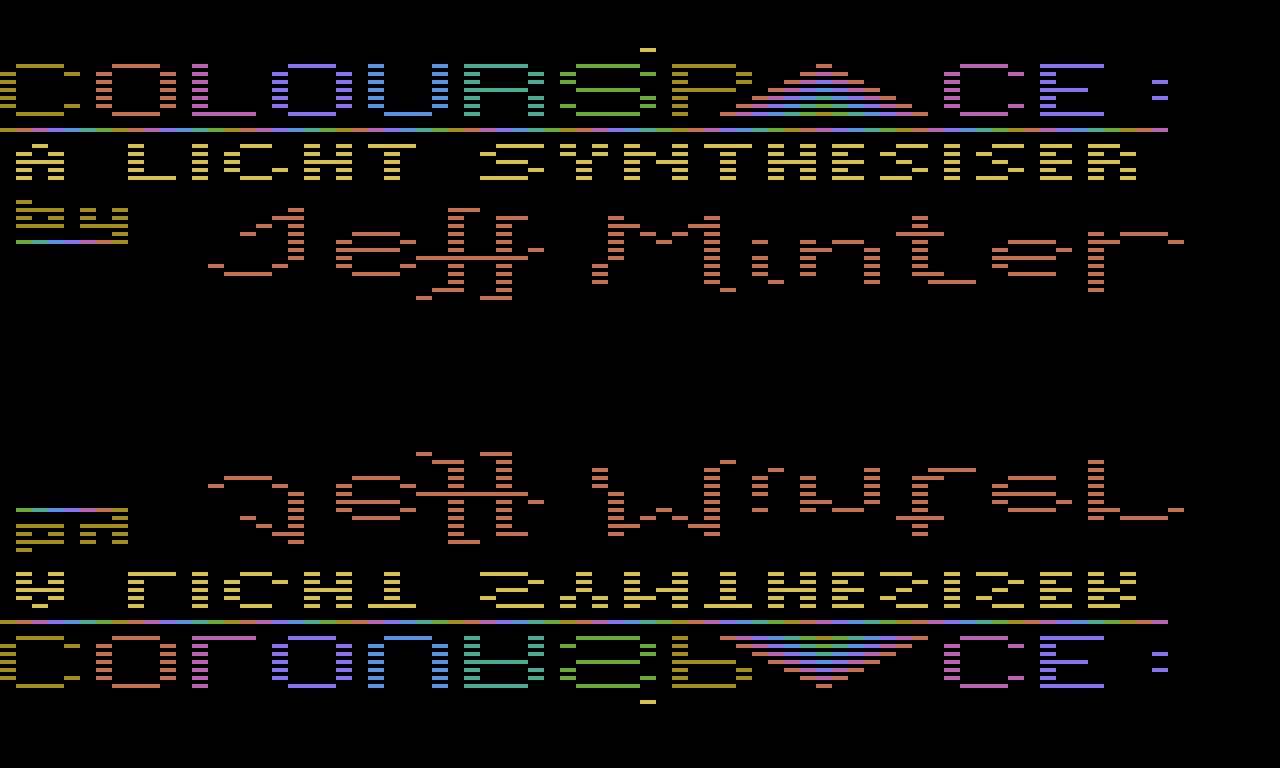
\includegraphics[width=12cm]{src/colorspace_painting/foregrounds/pixel_pattern_6.png}}%
    \end{adjustbox}
\caption{'Zarjax Interlace Res' Display Mode}
\end{figure}
\clearpage
